\documentclass{beamer}
\usetheme{Hannover}
%\usepackage{gb4e}
\usepackage{tipa}
\usepackage{ot-tableau}
\usepackage{phonrule}
\usepackage{hyperref}
\usepackage{graphicx}
\usepackage{comment}
\usepackage{tabularx}
\usepackage{verbatim}
\usepackage{ulem}

\addtobeamertemplate{navigation symbols}{}{%
    \usebeamerfont{footline}%
    \usebeamercolor[fg]{footline}%
    \hspace{1em}%
    \insertframenumber/\inserttotalframenumber
}

\newcounter{saveenumi}
\newcommand{\seti}{\setcounter{saveenumi}{\value{enumi}}}
\newcommand{\conti}{\setcounter{enumi}{\value{saveenumi}}}

\resetcounteronoverlays{saveenumi}


\title{Evidence for Prosodic Phrase Marking in French Double Negation}
\subtitle{An experimental approach}
\author{Jeremy Yeaton\\Viviane D\'eprez, PhD}
\institute{\'Ecole normale sup\'erieure de Paris\\Rutgers University}
\date{ConSOLE XXVI: UCL, London\\ February 16, 2018}

\begin{document}
\setbeamercovered{invisible}
\begin{frame}
\titlepage
\end{frame}

\begin{frame}
\frametitle{Nobody Say Nothing!}
\begin{enumerate}
%\pause
\item Negative \textbf{Concord}: A single negation reading of a sequence of Negative Concord Items (NCI)\\ \textit{Nobody say anything }\\
%\pause
\item Negative \textbf{Discord}: Double negation \\ 
\textit{Nobody say nothing $\rightarrow$ Everybody say something}
\end{enumerate}
%\pause
\bigskip
But French can do both:\\
\textit{Personne ne dit rien.}
\end{frame}

\begin{frame}
\label{contents}
\frametitle{Outline}
\tableofcontents
\end{frame}

\section{Background}
\begin{frame}
\frametitle{Macro-Parametric Theory}
\begin{block}{Generative Theoretical Stance}
NC languages are distinguished from DN ones by a macro-parameter \textit{(Zanutini 1991, Haegeman 1995, Zeijlstra 2004)}
\begin{itemize}
\item French, Spanish, Catalan, etc.: \textbf{NC Languages}
\item English, Dutch, German, etc.: \textbf{DN Languages}
\end{itemize}
\textbf{Predictions:} 
\begin{itemize}
\item No real NC/DN ambiguity in languages
\item DN Emerging in an NC language, or NC in a DN one would be a marked ``anomaly'', not part of the grammar
\end{itemize}
\end{block}
\end{frame}

\begin{frame}
\frametitle{The Nature of NCI}
\begin{block}{NCI are \textbf{non-negative} expressions}
NC reading from sentential negation (overt or covert):
\begin{itemize}
\item Indefinites \textit{(Zeijlstra 2004, Chierchia 2013)}\\
$\neg \exists x \exists y [$x said y$]$: Negated Indefinites\\
\item Universals \textit{(Giannakidou 2000, Shimoyama 2012)}\\
$\forall x \forall y \neg [$x said y$]$: Negated Universals
\end{itemize}
\textbf{Prediction:} No DN readings
\end{block}
%\pause
\begin{block}{NCI are \textbf{negative} expressions}
NC reading from Resumptive Quantification \textit{(May 1989, de Swart \& Sag 2002, D\'eprez 1997, 2000, 2011)}
\begin{itemize}
\item NO$<x,y>[$x said y$]$: Resumptive Quantification (NC)
\item NO$<x>$NO$<y>[$x said y$]$: Scopal interaction (DN)
\end{itemize}
\textbf{Prediction:} Both NC \& DN possible, but unclear why languages differ

\end{block}
\end{frame}

\begin{frame}
\frametitle{The Nature of NCI}
\begin{block}{NCIs are \textbf{ambiguous} expressions\\ (Micro-parametric approach)}
\begin{itemize}
\item Lexical ambiguity \textit{(Longobardi 1986)}
\item Structural ambiguity \textit{(D\'eprez 1997...2000)}\\
\begin{itemize}
\item $[_{DP} ... [_{NP} NCI ]]$: non-negative\\
\item $[_{DP} NCI [_{NP} ... ]]$: negative\\
\end{itemize}
D\'eprez 2011: \textsc{Neg} feature is interpretable at Phase Edge\\
If DP = phase, NCI = negative
\begin{enumerate}
\item At DP edge and
\item At vP or TP/CP edge
\end{enumerate}
If DP $\neq$ phase, only (2) matters
\item \textbf{Prediction:} NC \& DN subject to structural conditions, DP internal \& sentential, that can differ within and across languages
\end{itemize}
\end{block}
\end{frame}

\begin{frame}
\frametitle{The Case of French}
\begin{center}
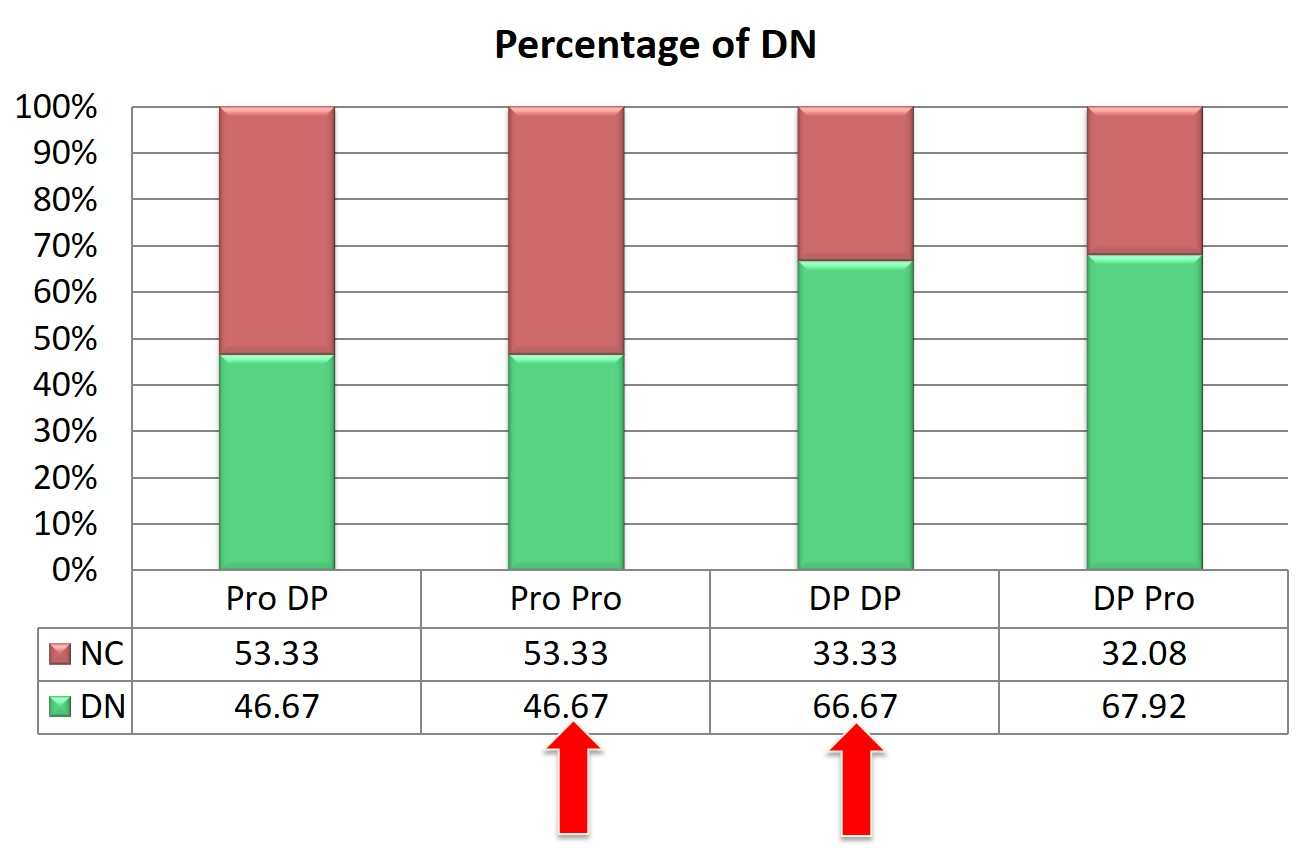
\includegraphics[width=\linewidth]{figures/syntax_and_structure.jpg}
\end{center}
D\'eprez et al, 2015, Picture choice task
\end{frame}
\begin{comment}
We saw that there was a slight preference for NC readings, but both were easily accepted, and in the PRO-PRO condition, participants responded at chance. in the DP subject conditions, there was even a preference for DN
\end{comment}

\begin{frame}
\frametitle{DN/NC and Prosody}
\begin{block}{Afrikaans \textit{(Huddlestone 2010)}:}
Results supporting a prosodic distinction between DN/NC readings
\end{block}
\begin{block}{Dutch \textit{(Fonville \& de Swart 2013)}:}
Mixed results: no characteristic prosody, but some patterns more closely associated with one type of reading\\
\textbf{Problem:} Design assumed context = accessed reading, no verification
\end{block}
\begin{block}{Catalan \textit{(Prieto et al 2013, Tubau et al 2015)}:}
Clear prosodic distinction in DN vs NC readings in answers to negative questions with NCI\\
\textbf{Problem:} In French, answers to negative questions with an NCI are not ambiguous: always DN
\end{block}
\end{frame}

\begin{frame}
\frametitle{French Prosody}
\begin{itemize}
\item No experimental evidence that prosody is a disambiguating factor in French, but some notes in the literature \textit{(Corblin 1996, Tovena \& Corblin 2008)}
\item French uses phrasing to mark focus \textit{(F\'ery 2000)}, indicated  by duration, intensity, and tone
\item In simple SVO sentences, \textit{Major Prosodic Phrases (MaP)} are identified by a pitch movement, a lengthening, or a pause \textit{(Avanzi et al, 2014)}
\end{itemize}
\end{frame}

\section{Research Questions}
\begin{frame}%
\frametitle{Research Question}
\begin{enumerate}
\item Is prosody used in disambiguating French transitive sentences with two NCIs?
\item What are the prosodic indicators which are employed by speakers to mark these differences?

\end{enumerate}
\end{frame}

\begin{frame}%
\frametitle{Predictions/ Hypotheses}
	\begin{enumerate}
	\item Like other languages (e.g.: Spanish, Catalan), the DN reading in French will be prosodically marked.
	\item Speakers will use a high pitch accent and extended duration to indicate this markedness.
	\end{enumerate}
\end{frame}

\section{Experimental Design}

\begin{frame}
\frametitle{General Idea}
\begin{itemize}
\item Native French speakers were presented with simple, ambiguous transitive sentences with one (Control) or two (Critical) NCIs in context
\item They were then asked to (at their own pace)
\begin{enumerate}
\item Read the entirety silently for comprehension
\item Read it aloud (as though to a child)
\item Respond to T/F question 
\end{enumerate}
\item Responses were recorded on an Asus Orion PRO gaming headset with a noise filtering microphone
\item Recording took place at the \textit{Laboratoire sur le Langage, le Cerveau, et la Cognition (L2C2)} in Bron, France
\item Total experimental time $\leq$ 20 minutes
\end{itemize}
\end{frame}

\begin{frame}
\frametitle{Some Examples}
\textbf{NC Context}
\begin{enumerate}
\item \textit{Dans notre famille, on est tous allergique \`a l'alcool :}\\
(In our family, we are all allergic to alcohol)
\seti
\end{enumerate}
\textbf{DN Context}
\begin{enumerate}
\conti
\item \textit{Chez les jeunes, la consommation d'alcool est effrayante :}\\
(Among the youth, the rate of alcohol consumption is frightening)
\seti
\end{enumerate}
\textbf{Ambiguous Critical Item}
\begin{enumerate}
\conti
\item \alert{\textbf{Personne ne boit rien dans les soir\'ees.}}\\
(Nobody drinks nothing/ anything at parties)
\seti
\end{enumerate}
\textbf{Interpretation Verification}
\begin{enumerate}
\conti
\item \textit{Ils ne boivent pas d'alcool.}\\
(They don't drink alcohol)\\
= \textbf{T} for NC interpretation\\
= \textbf{F} or DN interpretation
\end{enumerate}
\end{frame}

\begin{frame}
\frametitle{Stimuli}
\begin{itemize}
\item 40 total context/sentence pairs (8 items $\times$ 5 conditions):
\begin{enumerate}
\item 8 $\times$ \textbf{Double Negative:} \textit{\alert{Personne} ne mange \alert{rien} ici}
\item 8 $\times$ \textbf{Negative Concord:} \textit{\alert{Personne} ne mange \alert{rien} ici}
\item8 $\times$ \textbf{Negative Object:} \textit{Marie ne mange \alert{rien} ici}
\item8 $\times$ \textbf{Negative Subject:} \textit{\alert{Personne} ne mange mie ici}
\item 8 $\times$ \textbf{Fillers}
\end{enumerate}
\item Pseudorandomized
\item Same 8 frequent monosyllabic verbs
\item Same number of syllables in target sentence
\item Maximized sonorant use where possible
\item Final PP to avoid sentence boundary L tone on object NCI
\end{itemize}
\end{frame}

\begin{frame}
\frametitle{Participants}
\begin{itemize}
\item 20 native French speakers (M=4)
\item Age 18-45 (mostly students at University of Lyon)
\item Representative of diverse regions of France
\item All had a minimum of a university degree
\end{itemize}
\end{frame}

\begin{frame}
\frametitle{Data}
\begin{center}
\begin{tabular}{ l l l l }
\textbf{Condition} &\textbf{Structure}& \textbf{Abbreviation} & \textbf{n} \\
\hline
Double Negation &NCI-NCI & DN & 137 \\
Negative Concord & NCI-NCI& NC & 140 \\
\hline
\textbf{Subtotal Criticals} & && 277 \\
\hline
Single Negative Object &DP-NCI &NegOb & 149 \\
Single Negative Subject & NCI-DP&NegSub & 149 \\
\hline 
\hline
\textbf{Total} & && 575\\
\end{tabular}
\end{center}

\end{frame}

\begin{frame}
\frametitle{Analysis}
\begin{itemize}
\item Utterances were excised from context and text-aligned using \textbf{EasyAlign} \textit{(J.-Ph. Goldman, 2011)} in \textbf{Praat} \textit{(Boersma \& Weenink, 2015)}
\item Extracted for each syllable using \textbf{ProsodyPro} \textit{(Xu, 2013)}:
\begin{itemize}
\item Duration
\item Max F0
\item Min F0
\item 10 time-normalized F0 measurements
\end{itemize}
\item Only the first 6 syllables are included:\\ \textit{per sonne ne [verb] rien PP$[1]$}
\item F0 values were de-meaned
\item Analysis performed in R (LM, LMEM)
\item Removed 1,136/33,790 ($3.4\%$) data points \\$\geq3\sigma$ from $\mu$
\end{itemize}
\end{frame}


\section{Results}

\begin{frame}
\frametitle{Behavioral Overview}
\begin{tabular}{ll}
  \begin{tabular}{l}
  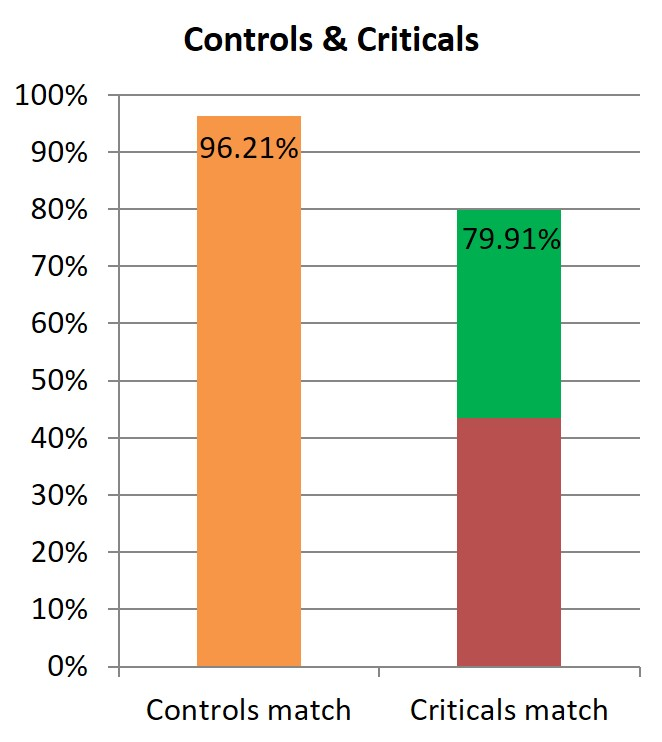
\includegraphics[width=0.43\linewidth]{figures/context_controls.jpg}
  \end{tabular}
  & \begin{tabular}{l}
 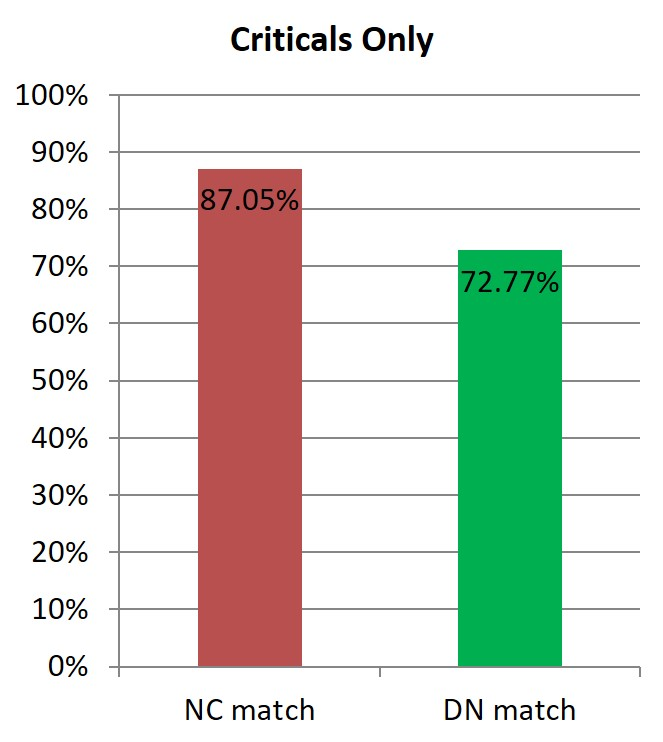
\includegraphics[width=0.43\linewidth]{figures/context_criticals.jpg}
  \end{tabular}
\end{tabular}
\end{frame}

\begin{frame}
\frametitle{Behavioral Overview}
\begin{center}
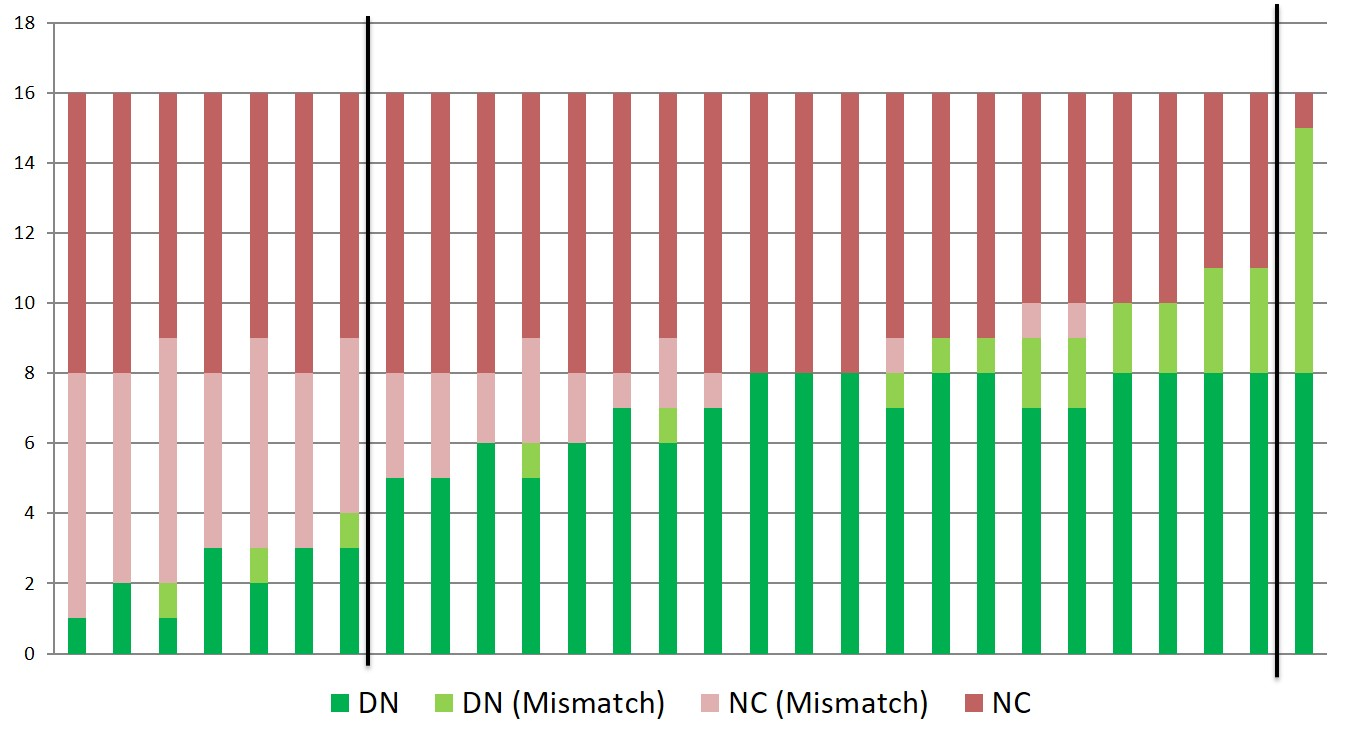
\includegraphics[width=\linewidth]{figures/results_by_subject.jpg}
\end{center}
\end{frame}

\begin{frame}
\frametitle{Duration}
\begin{center}
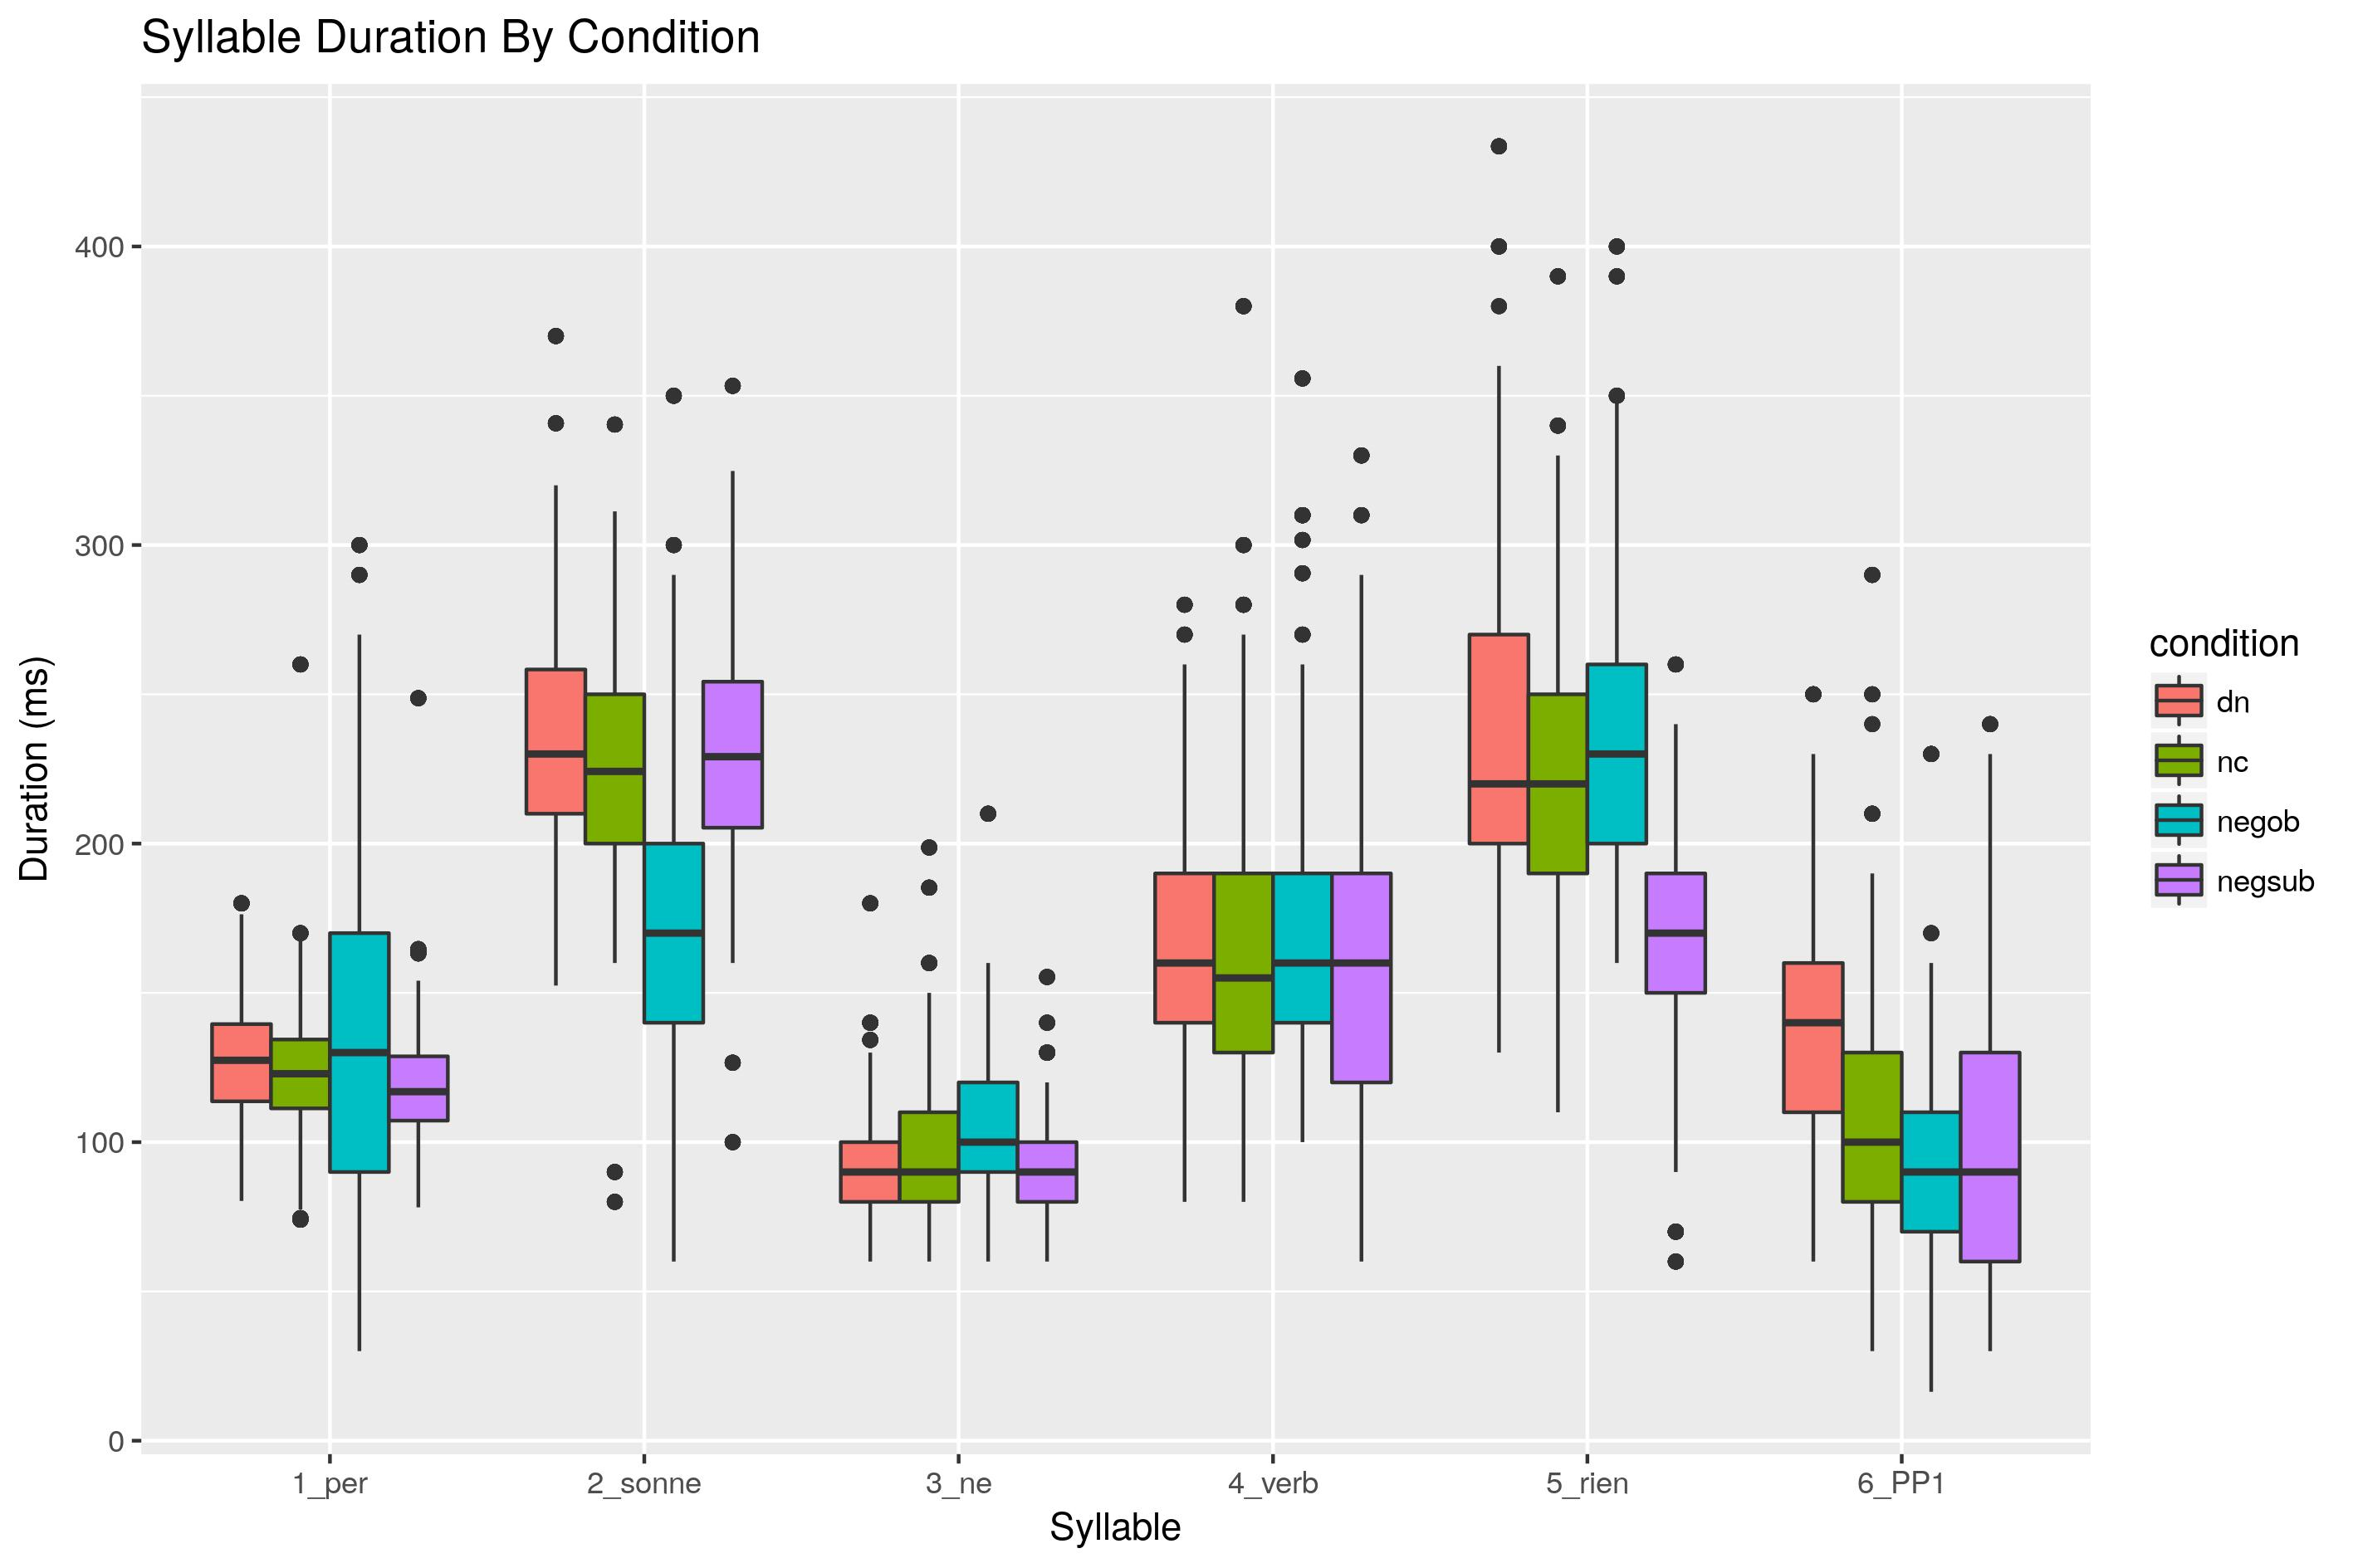
\includegraphics[width=\linewidth]{figures/overall_dur.jpeg}
\end{center}
\end{frame}

\begin{frame}
\frametitle{Duration}
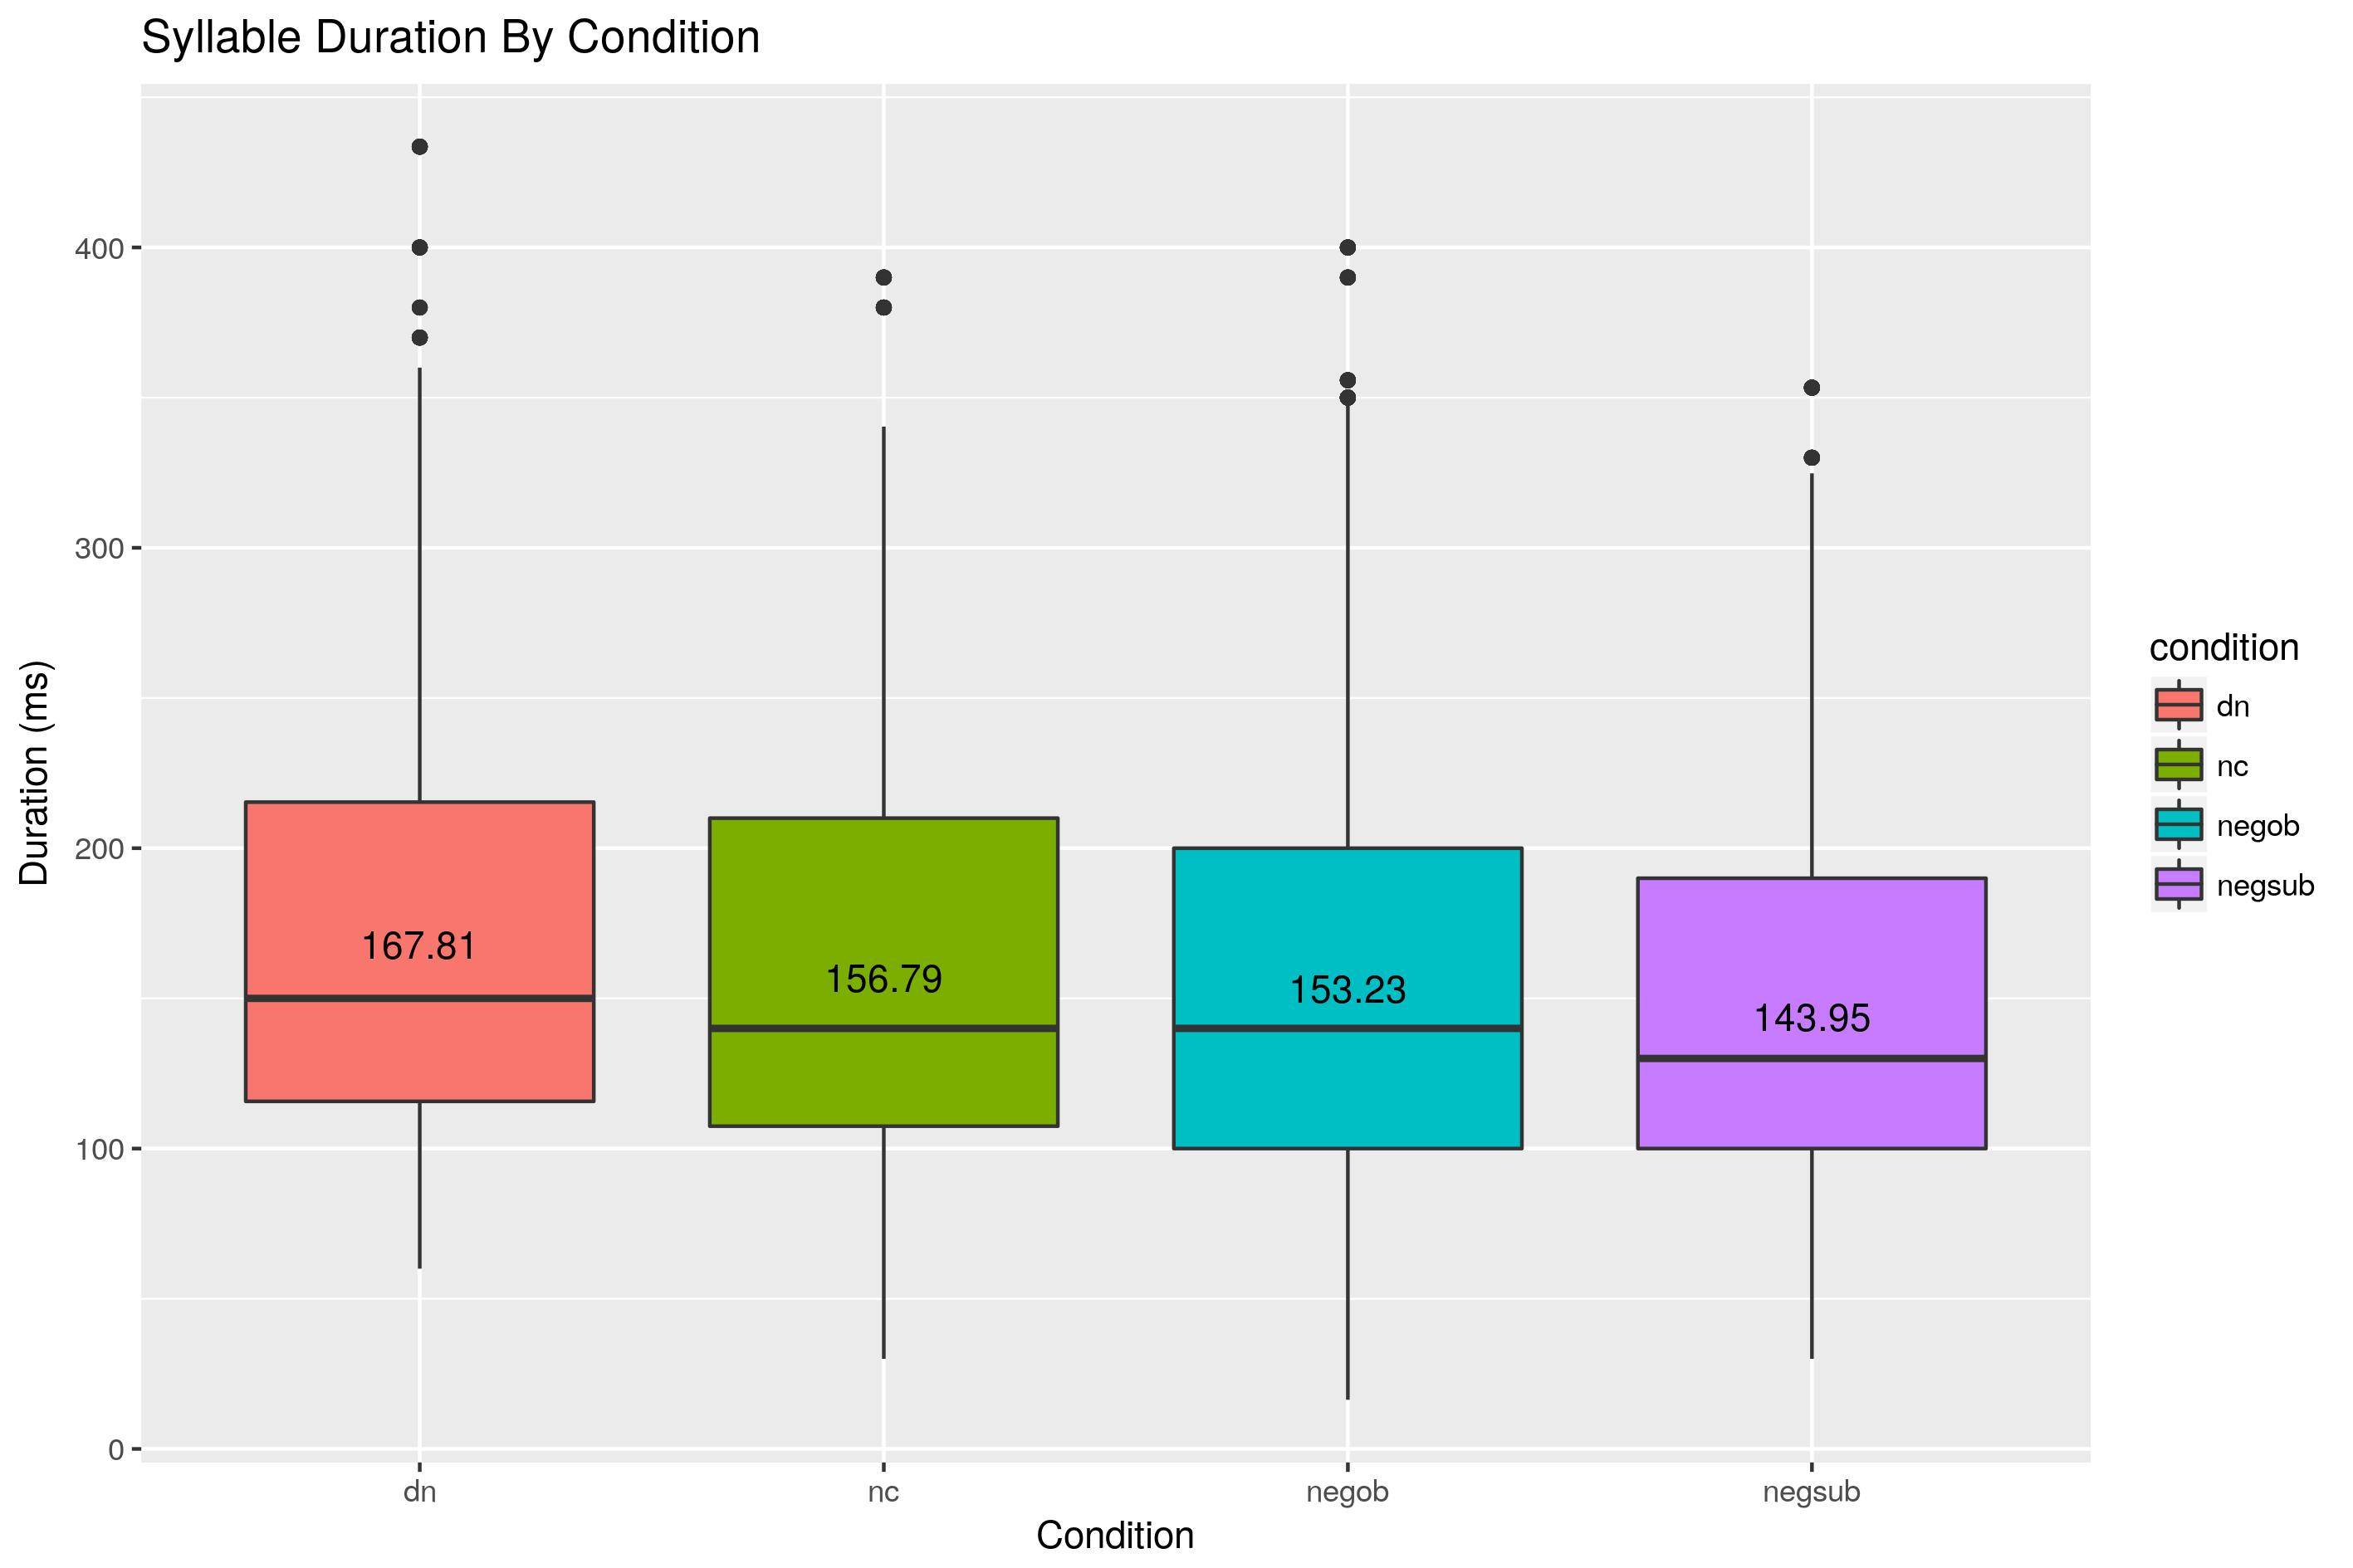
\includegraphics[width=\linewidth]{figures/dur_cond.jpeg} 
\end{frame}

\begin{frame}
\frametitle{Range by Syllable}
\begin{center}
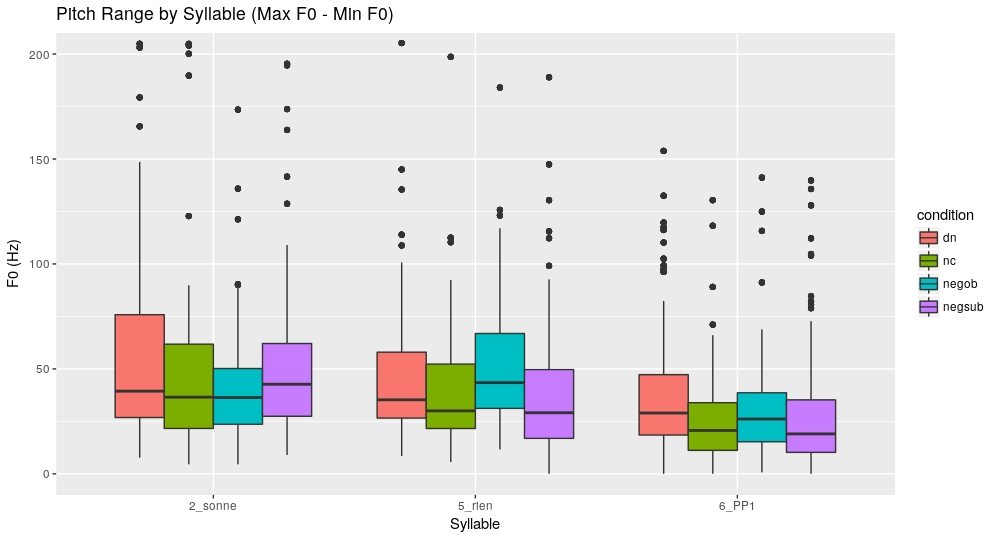
\includegraphics[width=\linewidth]{figures/pitch_range.jpeg}
\end{center}
\end{frame}

\begin{frame}
\frametitle{Pitch Contours by Subject}
\begin{center}
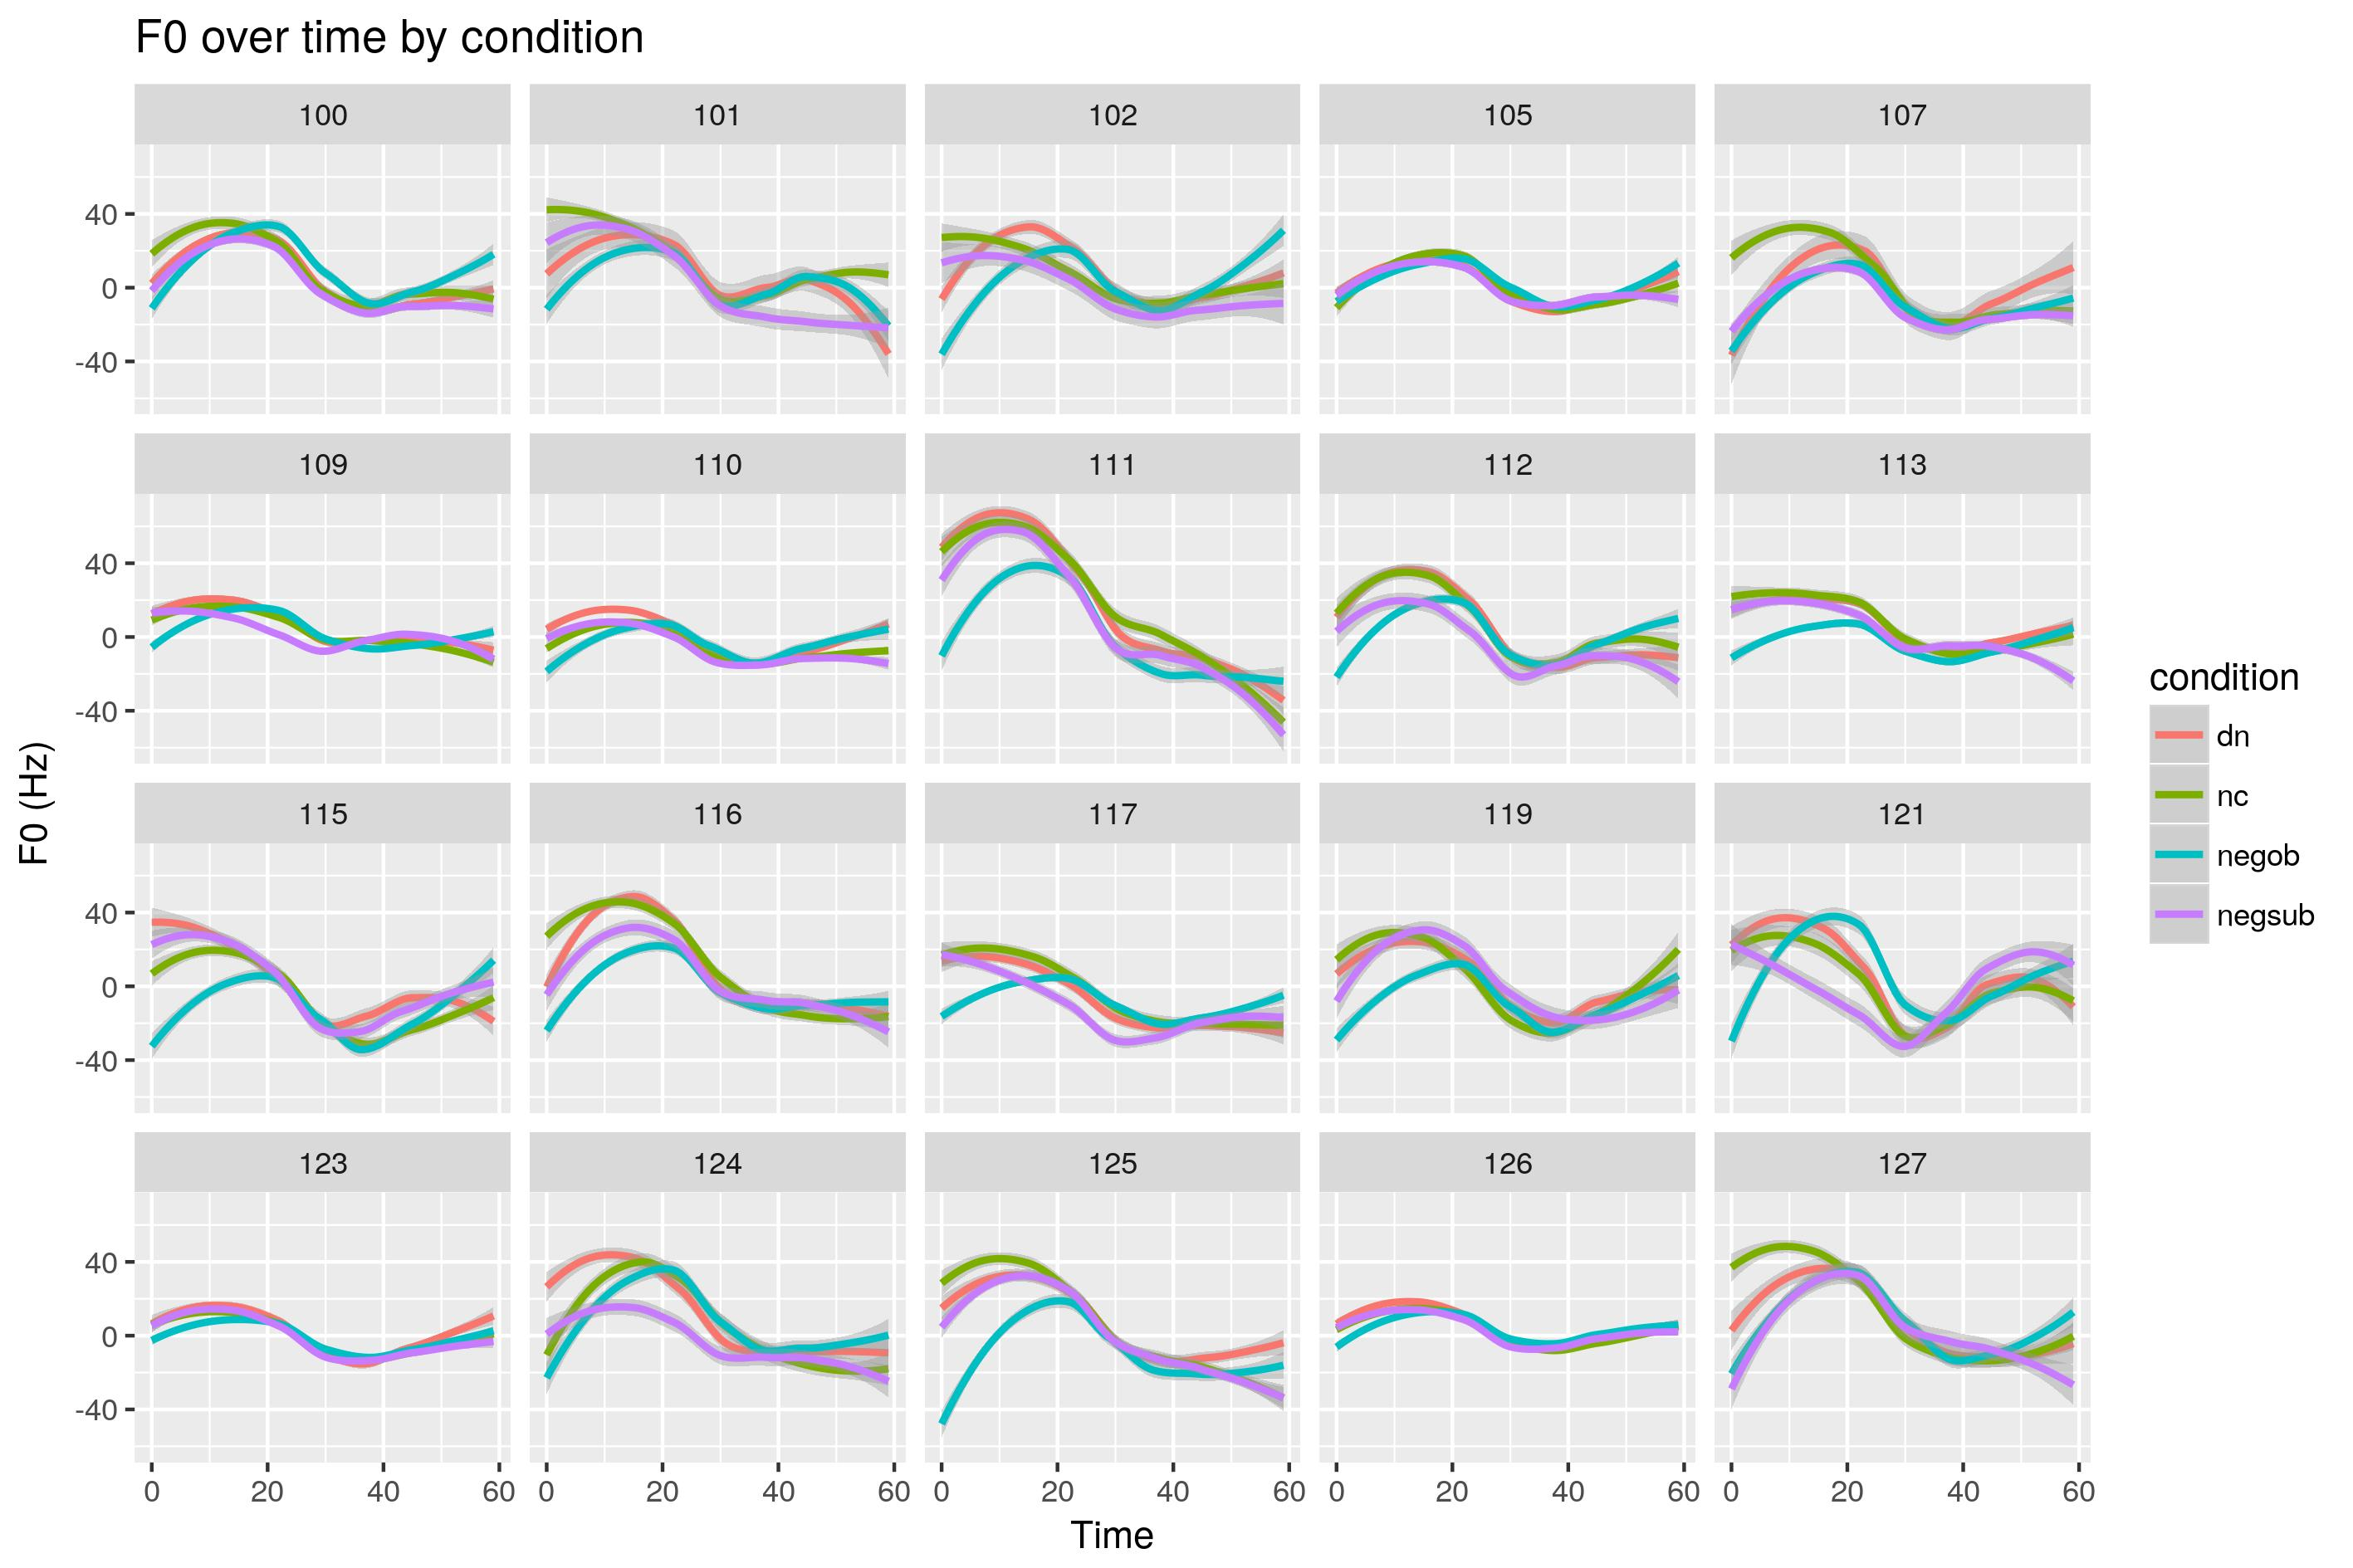
\includegraphics[width=\linewidth]{figures/overall_facet.jpeg}
\end{center}
\end{frame}

\begin{frame}
\frametitle{Aggregated Pitch Contours}
\begin{center}
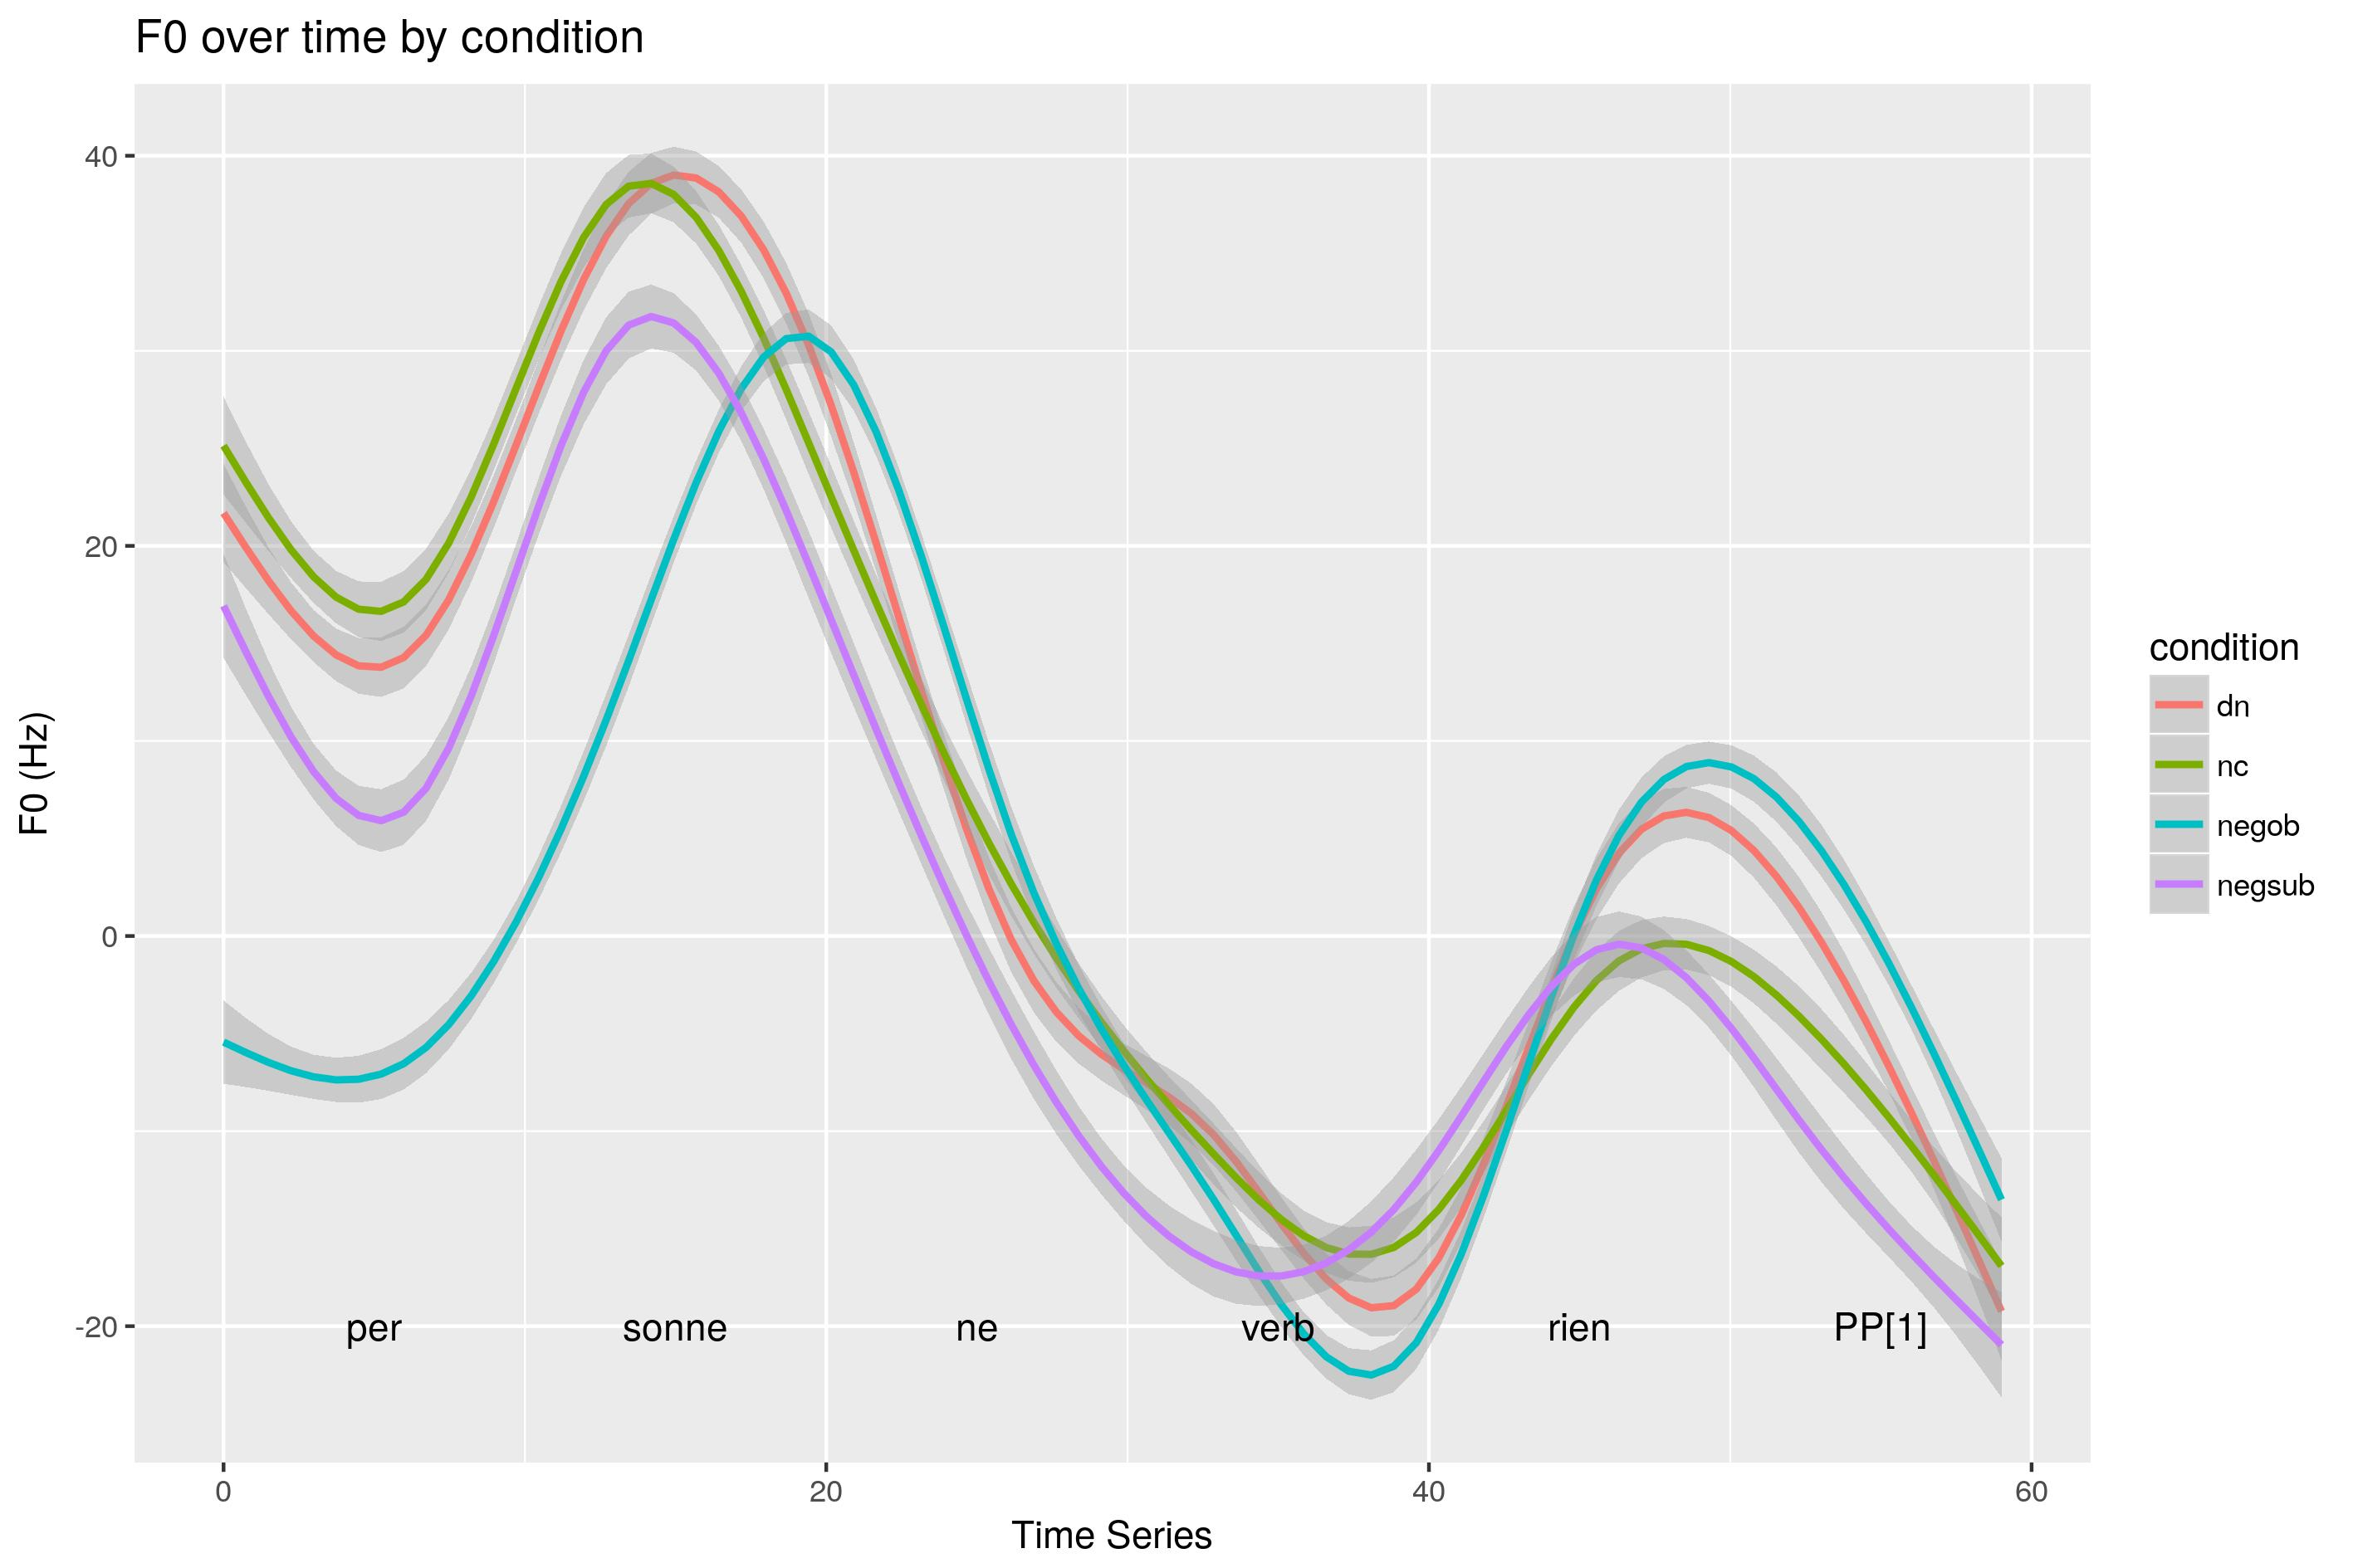
\includegraphics[width=\linewidth]{figures/overall_pitch.jpeg}
\end{center}
\end{frame}

\begin{frame}
\frametitle{A Closer Look}
\begin{center}
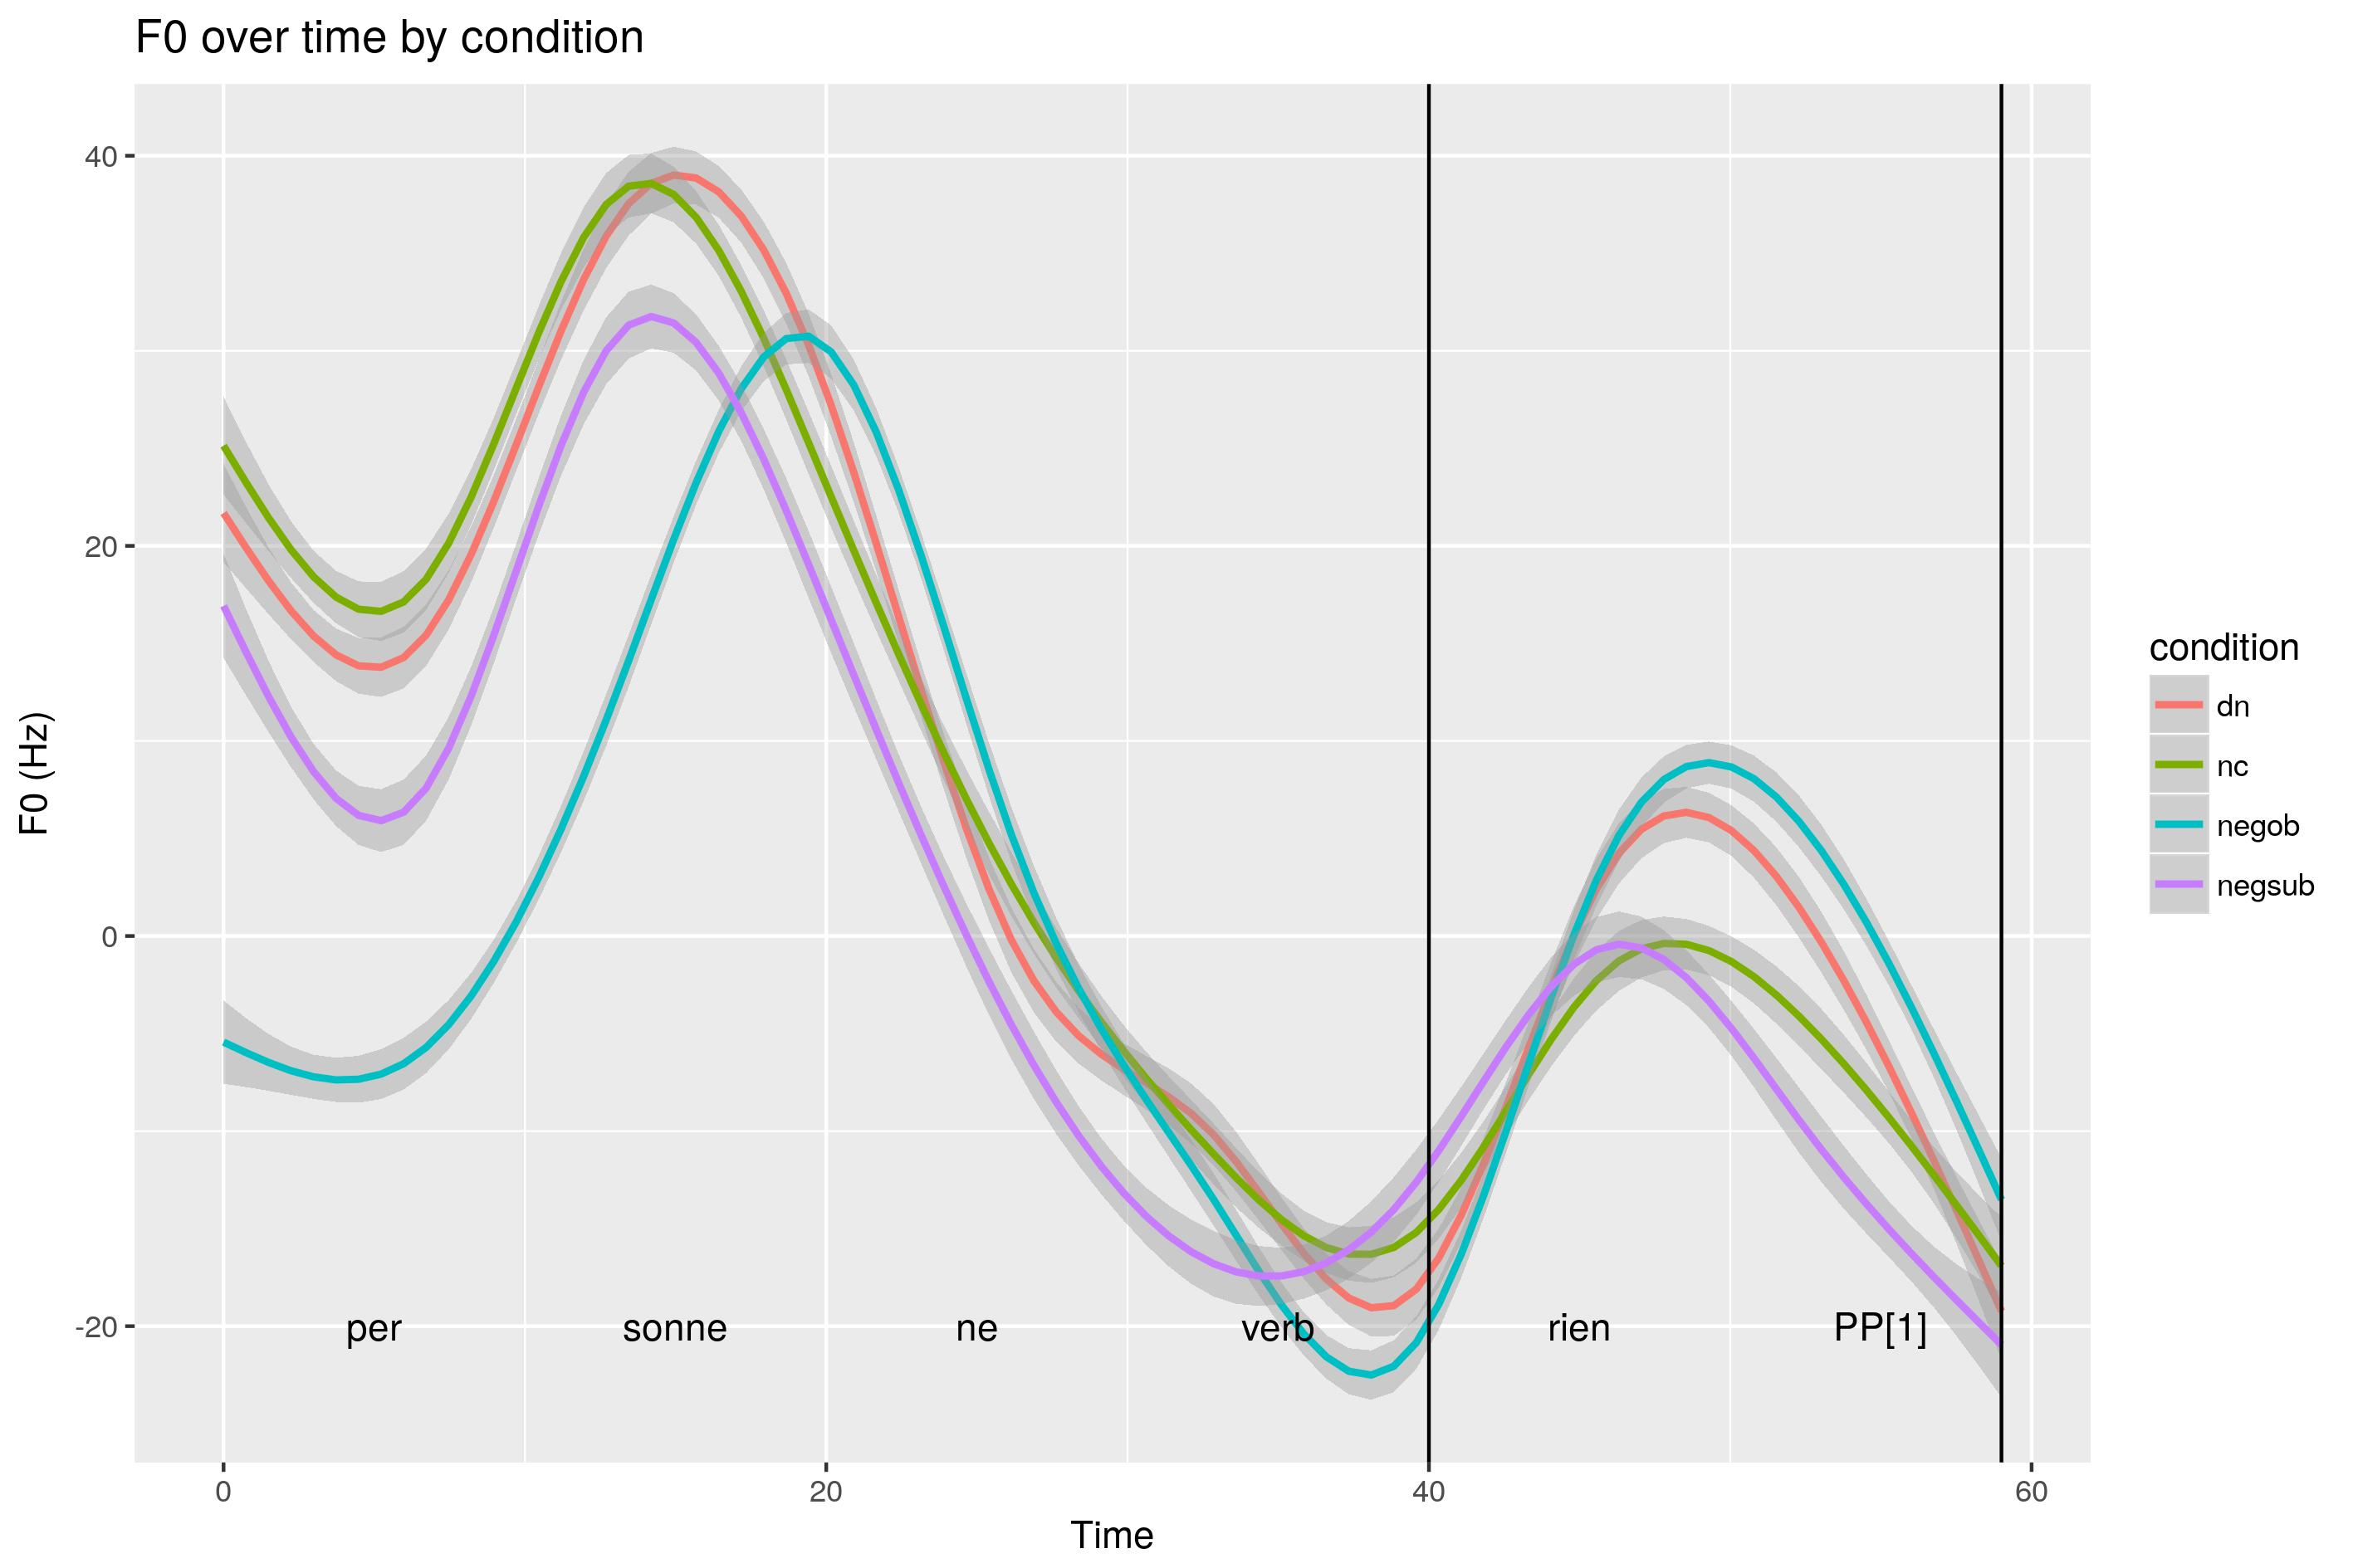
\includegraphics[width=\linewidth]{figures/overall_pitch_z.jpeg}
\end{center}
\end{frame}

\begin{frame}
\frametitle{A Closer Look}
\begin{center}
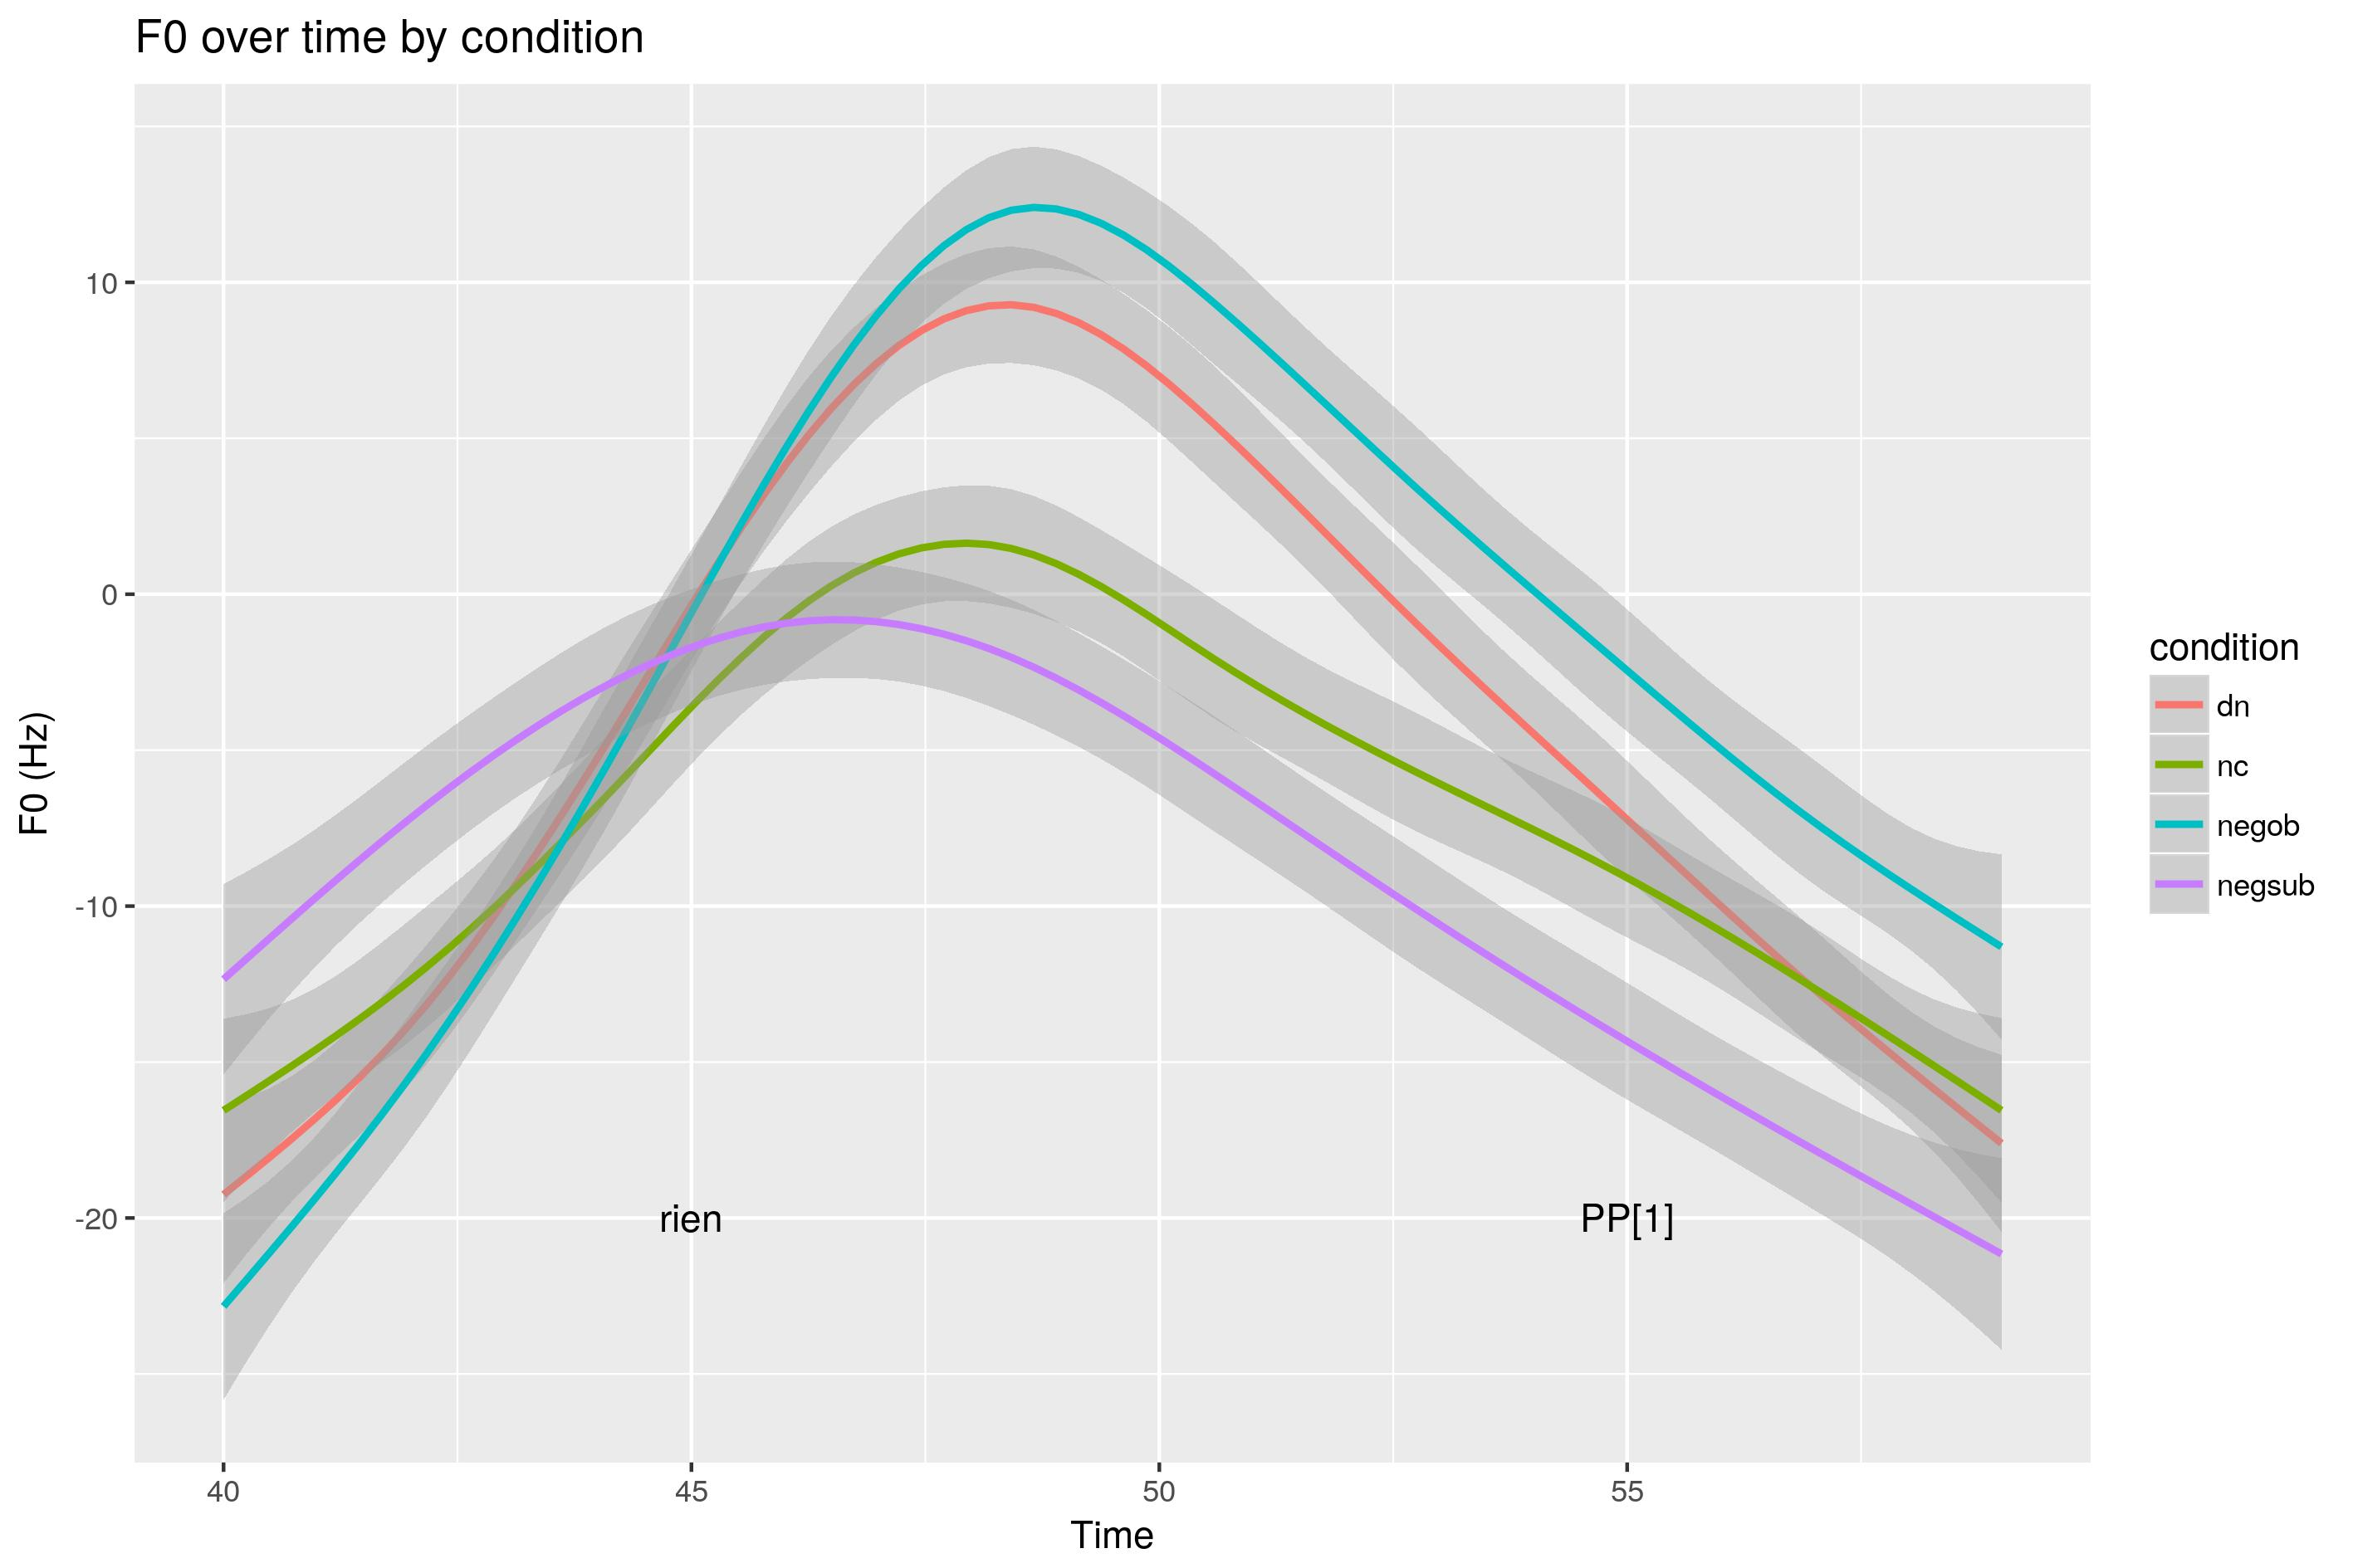
\includegraphics[width=\linewidth]{figures/f0_zoomed.jpeg}
\end{center}
\end{frame}

\begin{frame}
\frametitle{A Closer Look}
\begin{center}
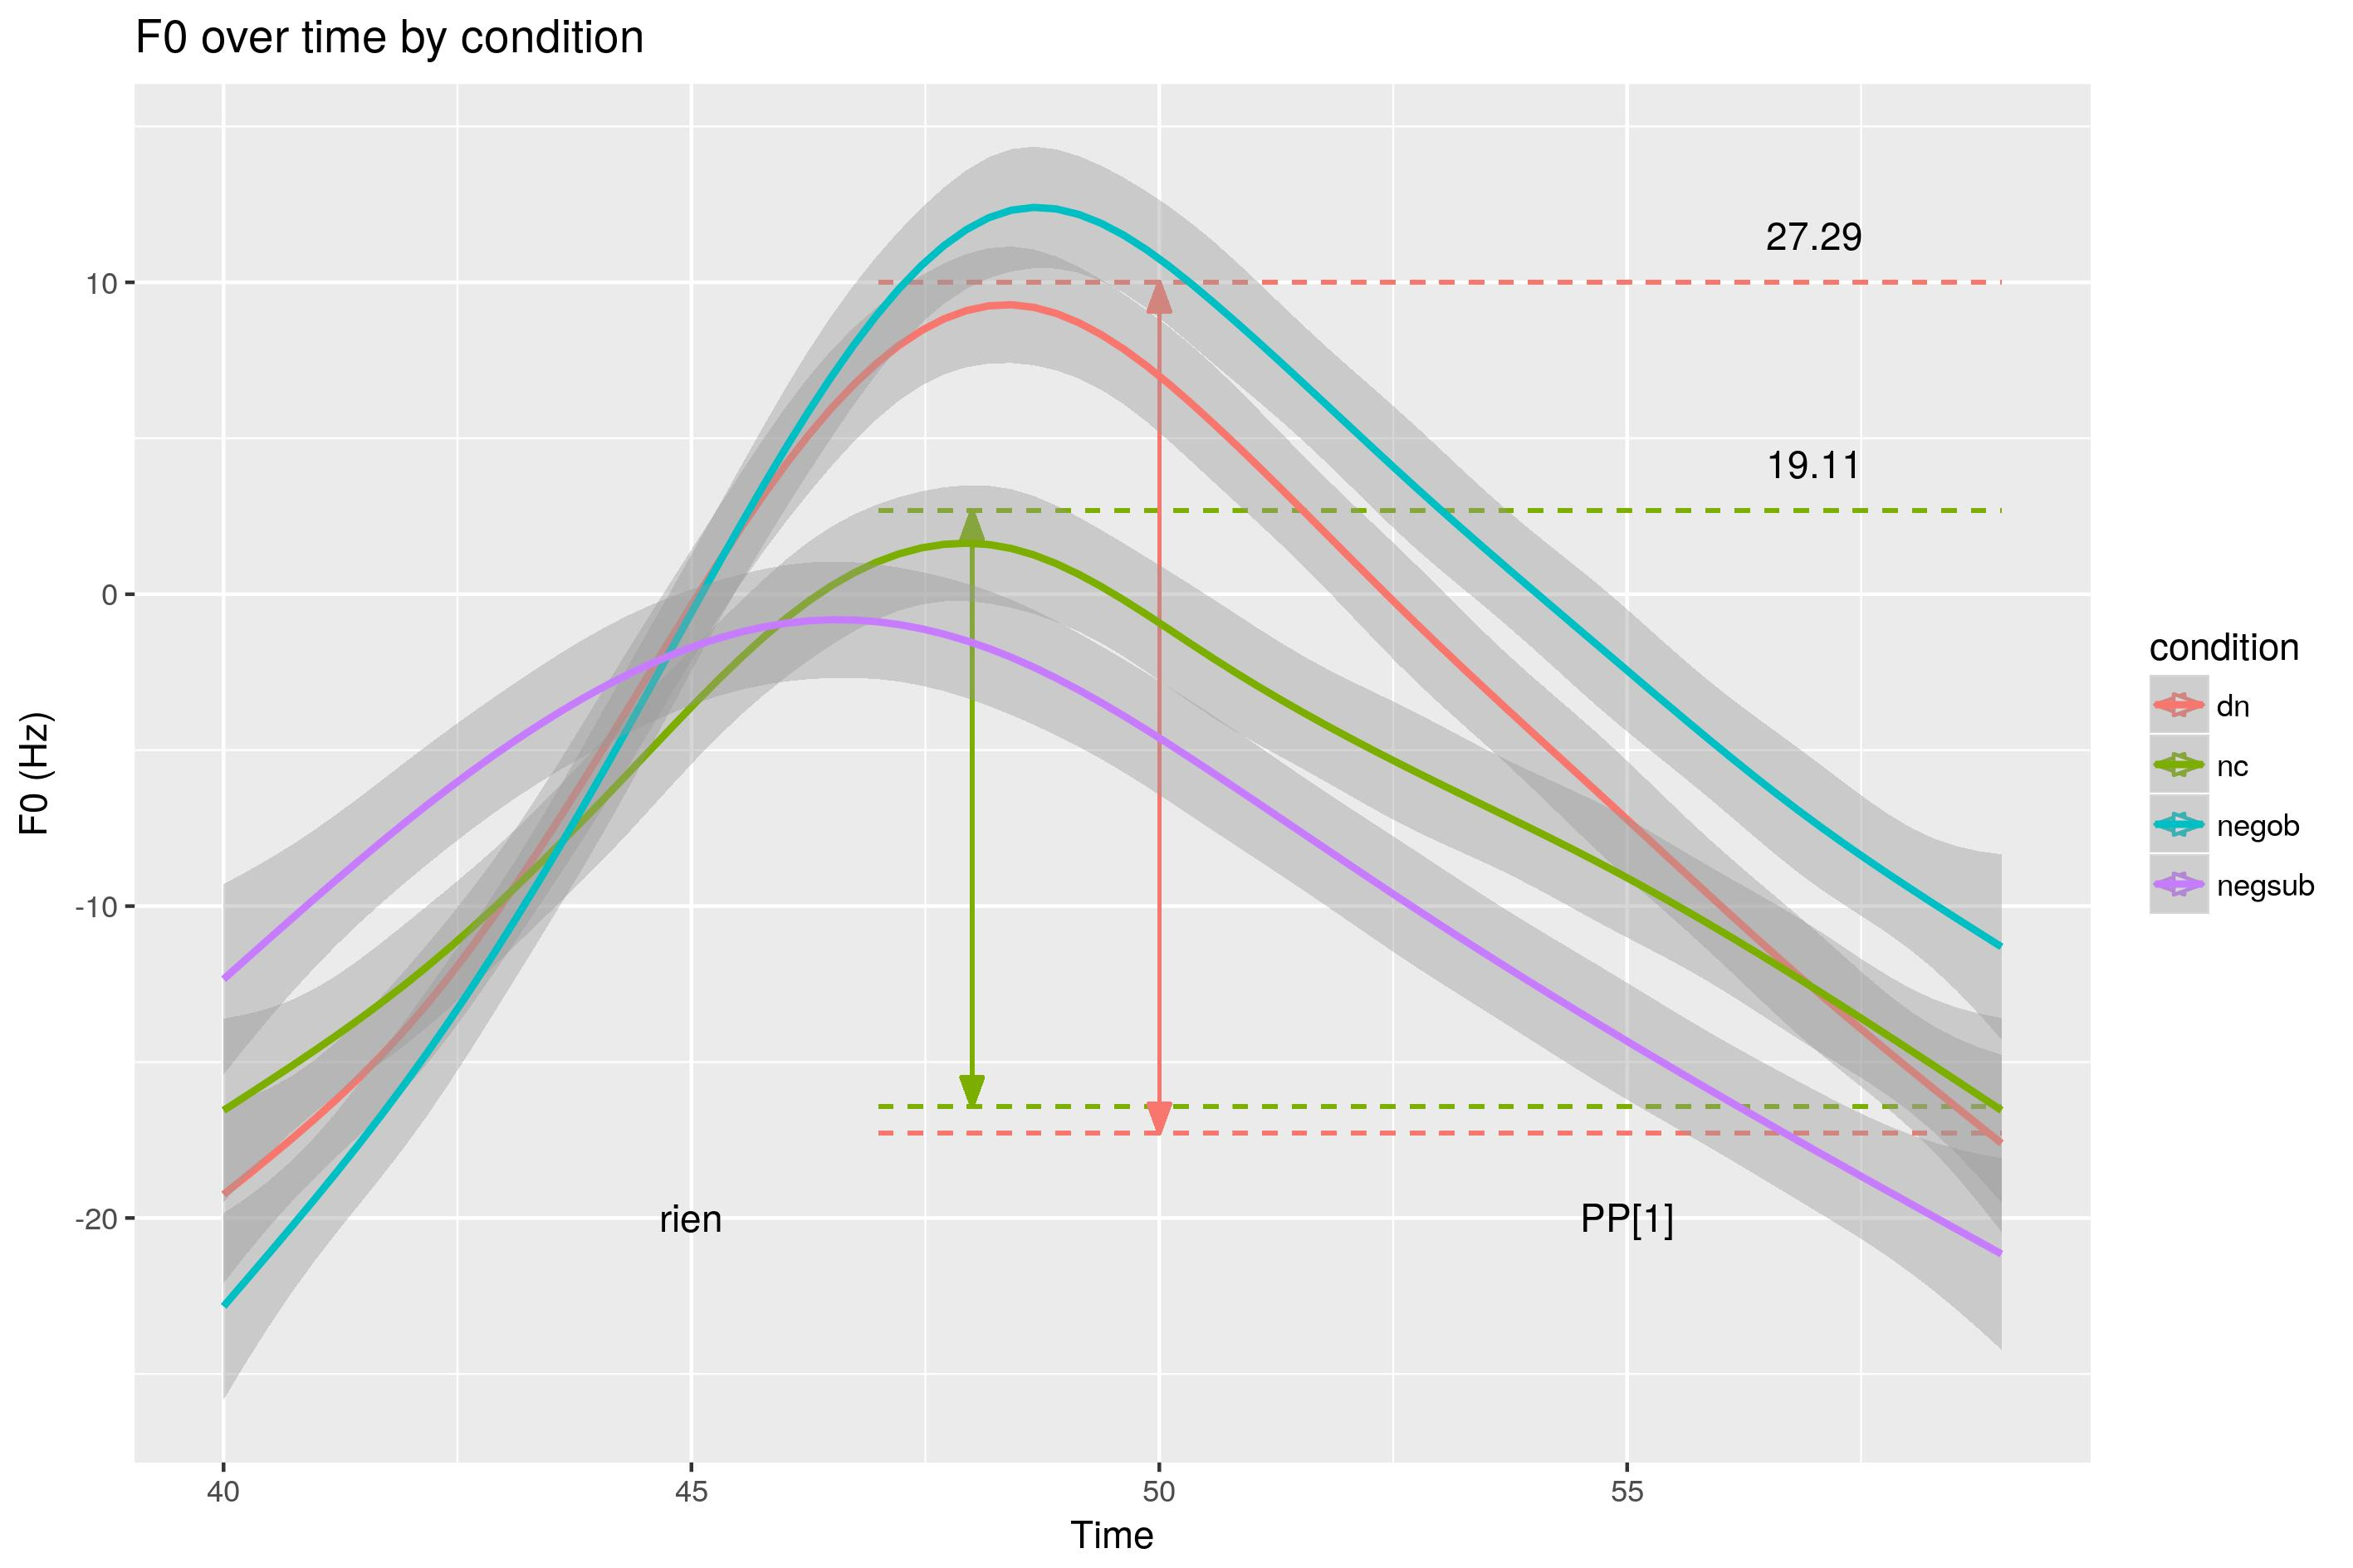
\includegraphics[width=\linewidth]{figures/zoomed_triangles.jpeg}
\end{center}
\end{frame}

\begin{frame}
\frametitle{NC Flattening}
\label{lm}
\begin{block}{Linear Model:}
$F0$ $\tilde{}$  $time series + condition + time \times condition$
	\begin{enumerate}
	\item Interaction effect of $time series \times condition$: \\ 
	\textbf{NC} $(t= -4.558,p=5.25e-06)$***\\\textbf{NegSub} $(t=4.011,p=6.11e-05)$***\\\textbf{NegOb} $(t=2.549,p=0.0108)$*
	\item Main effect of $condition$:\\
	 \textbf{NC} $(t=-5.077,p=3.93e-07)$***\\ \textbf{NegSub} $(t=-4.771,p=1.87e-06)$***\\ \textbf{NegOb} $(t=-2.006,p=0.0449)$*
	\item Significant effect of $time series$ across conditions
	\end{enumerate}
\end{block}
\hyperlink{routput}{\beamerbutton{LM}}
\hyperlink{routput:lmem}{\beamerbutton{LMEM}}
\hyperlink{routput:anova}{\beamerbutton{ANOVA}}
\end{frame}


\section{Discussion}
\begin{frame}
\frametitle{Back to the Research Questions}
\begin{enumerate}
\item Is prosody used in disambiguating French transitive sentences with two NCIs?
\item What are the prosodic indicators which are employed by speakers to mark these differences?
\end{enumerate}
\end{frame}

\begin{frame}
\frametitle{Circling Back to the Predictions}
\begin{enumerate}
\item Like other languages (e.g.: Spanish, Catalan), the DN reading in French will be prosodically marked.
\item Speakers will use a high pitch accent and extended duration to indicate this markedness.
\end{enumerate}
\end{frame}

\begin{frame}
\frametitle{Discussion: Duration}
\begin{itemize}
\item Avanzi found that separate O phrasing is correlated with articulation rate (syllable duration)
\item Extended duration in DN condition is encouraging for our hypothesis that NCI$_{2}$ is phrased separately
\end{itemize}
\end{frame}

\begin{frame}
\frametitle{Discussion: F0}
The F0 distinctions we see on the second NCI are realizations of phrasing and tone:
\begin{block}{NC}
\begin{itemize}
\item Focus on \textit{personne}
\item \textit{rien} is phrased as part of VP\\
L*\hspace{1.7cm} H-\hspace{.8cm} L* \hspace{.5cm}\alert{H-/L-} \hspace{1.2cm}L\%\\
\small{(($[_{DP}$\textbf{Personne}$]_{AP})([_{VP}$ne V \textbf{rien}$]_{AP})...([_{PP}...$PP$...]_{AP})_{IP})$}
\end{itemize}
\end{block}
%\pause
\begin{block}{DN}
\begin{itemize}
\item Focus on \textit{personne}
\item VP is ``dephrased'' \textit{(F\'ery 2010)}
\item Focus on \textit{rien}, which forms its own phrase\\
L* \hspace{1.7cm}H-\hspace{.5cm} L* \hspace{.8cm}\alert{LH-} \hspace{1.6cm}L\%\\
\small{(($[_{DP}$\textbf{Personne}$]_{AP})$ ne V $([_{DP}$\textbf{rien}$]_{AP})...([_{PP}...$PP$...]_{AP})_{IP})$}
\end{itemize}
\end{block}
\end{frame}

\section{Conclusions}
\begin{frame}
\frametitle{Conclusions}
\begin{itemize}
\item The availability of both readings rules out a Macro-Parametric approach
\item This could support either a Resumptive Quantification approach or a Micro-Parametric one
\item The acoustic cues that we see in French to mark phrasing might be clues to Syntax:
\begin{itemize}
\item \textbf{NC:} NCI$_{2}$ is phrased within the VP \& has H-\\
$[_{TP}$Personne $[$ne dit $[_{vP}[_{VP}$\sout{dit} \alert{rien}$]]]]$\\
\textit{NCI$_{2}$ remains inside VP, so its \textsc{Neg} feature is not interpretable since it is not at an edge}
\item \textbf{DN:} NCI$_{2}$ forms its own prosodic phrase with LH-\\
$[_{TP}$Personne $[$\textit{ne dit} $[_{vP}$ \alert{rien} $[_{VP}$ \sout{rien} $]]]]$\\
\textit{NCI$_{2}$ is at vP edge where its \textsc{Neg} feature is interpretable}
\end{itemize}
\end{itemize}
\end{frame}
\begin{frame}
\frametitle{Outstanding Questions\\ and Next Steps}
\begin{itemize}
\item Are these differences actually perceptible to speakers?
\item Might speakers emphasize these features more in a situation with less clear context?
\item Could these strategies be employed with \textit{less ambiguous} types of multiple NCI sequences to the same effect?
\item How can we investigate the processing of these different readings with an ERP study? Does one have a higher cost?
\end{itemize}
\end{frame}

\begin{frame}
\begin{center}
\frametitle{Thank you for your attention!}
\begin{block}{Acknowledgements}
Dr. Fanny Meunier, CNRS, L2C2\\
French Embassy in the U.S.\\
Rutgers Comparative and Experimental Linguistics Lab\\
Aresty Center for Undergraduate Research\\
\end{block}

\bigskip

\begin{tabular}{l r}

\includegraphics[width=.25\linewidth]{figures/psl.png} & 
\includegraphics[width=.25\linewidth]{figures/rutgers.jpeg} \\
\end{tabular}
\bigskip

\end{center}
\small{\url{jdyeaton27@gmail.com}}
\end{frame}

\begin{frame}
\frametitle{R Output: Linear Model}
\label{routput:lm}
\tiny\verbatiminput{figures/lm.result}
\hyperlink{lm}{\beamerbutton{Back to results}}
\end{frame}

\begin{frame}
\frametitle{R Output: LMEM}
\label{routput:lmem}
\tiny\verbatiminput{figures/lmem.result}
\hyperlink{lm}{\beamerbutton{Back to results}}
\end{frame}

\begin{frame}
\frametitle{R Output: ANOVA}
\label{routput:anova}
\tiny\verbatiminput{figures/anova.result}
\hyperlink{lm}{\beamerbutton{Back to results}}
\end{frame}

\end{document}

%Abstract
\begin{comment}
Evidence for Prosodic Phrase Marking in French Double Negation
Introduction. Among languages which readily facilitate Negative Concord (NC), that is, a single negation reading of a sequence of Negative Concord Items (NCI) (1c), French is problematic because it also readily accepts Double Negative (DN) interpretations of the same sequences. This DN interpretation is considered to be marked (De Swart, Corblin, 1996), however a cross-linguistic picture choice task (Deprez et al, 2015) found that these DN readings arise much more than previously thought, and can, in fact, sometimes be preferred. By contrast, other, stricter NC languages (e.g.: Catalan, Spanish), have a much higher proportion of NC responses. The picture choice task in French found that parallel pronominal (personne, rien) NCI sequences resulted in an at-chance ratio between NC and DN. A further study found that, given the same NCI sequence (1c) in contrasting context (1a & 1b), speakers will interpret according to the context about 80\% of the time (Deprez & Yeaton, 2017). The extent to which prosody plays a role in such interpretations has been investigated in Catalan, Spanish, and Dutch (Tubau et al, 2015; Prieto et al, 2013; Fonville, 2013). Prior to the present study, there have been only informal notes in the literature (Corblin 1996, Tovena&Corblin 2008) pointing to prosody as a disambiguating factor in French. The present study seeks to fill this gap in experimental evidence to investigate the role of prosody in disambiguating French transitive sentences with two NCI.
Method. Recordings of 20 native French speakers reading simple transitive sentences containing one (control) or two (critical) NCIs were used in the analysis presented. Participants were presented with a brief context (1a, 1b), then sentences (1c) on a screen which they would first read silently, then aloud, then respond to a T/F statement (1d) to ensure that their interpretation matched the presented context. Only context matching interpretations were used in the prosody analysis. The target transitive sentences were excised from context and analyzed using Praat. Duration, intensity, and 10 time-normalized f0 measurements were taken for each syllable. R was used to conduct t-tests comparing syllable duration and f0 for each of the time normalized windows between conditions.
Results. For the purposes of this analysis, only the first 6 syllable of the utterance were used (per/sonne/ ne/ [verb]/ rien/ + 1/[PP]). F0 values were scaled to normalize for subject range variance. Comparison of f0 values between conditions found a significant difference (p<.05) between the NC and DN conditions on the object as well as the following syllable. Comparison to the control conditions found that the NC interpretations manifest a systematic flattening of pitch in the same syllables, whereas the DN condition closely matches the single negative object condition. A significantly different duration between the DN and NC interpretations was found for the object and following syllable (p<.05). Further analyses are ongoing. Our results confirm that prosody plays a role in distinguishing NC&DN readings. We argue for a distinction in phrasing.
Sample disambiguating contexts & critical item.
(1) a. Dans notre famille, on est tous allergique à l'alcool :      NC Context
        (In our family, we are all allergic to alcohol)     
    b, Chez les jeunes, la consommation d’alcool est effrayante:    DN Context
        (In the youth population, alcohol consumption is frightening)  
    c.  Personne ne boit rien dans les soirées.            Critical test Item
         (Nobody drinks anything/nothing at parties)
    d.  Ils ne boivent pas d’alcool.                 Interpretation verification sentence
        (They don’t drink alcohool)    T for (1a)/F for (1b) 
\end{comment}

\begin{frame}
\frametitle{Duration}
\begin{tabular}{ll}
\begin{tabular}{lll}
Condition & Mean (ms) & $\sigma$\\
\hline
DN & 167.81 & 63.42\\
NC & 156.79 & 65.15\\
NegOb&153.23&65.70\\
NegSub&143.95&59.88\\
\end{tabular}
\end{tabular}
\end{frame}
